\section{Evaluasi}
\label{sec:evaluasi}

Bagian ini memaparkan mengenai sistem yang sudah dibuat, pengujian yang dilakukan untuk memastikan sistem bekerja sesuai dengan yang diharapkan, serta analisis \textit{benchmark} yang dilakukan. Pengujian dilakukan dengan menggunakan sistem yang telah diimplementasikan pada Bagian \ref{sec:implementation}. Evaluasi bertujuan untuk mendapatkan hasil analisis sesuai rumusan masalah yang telah ditetapkan pada Bagian \ref{sec:rumusan-masalah}. Evaluasi akan dibagi menjadi tiga bagian, yaitu penjelasan terkait \textit{setup} dan konfigurasi yang digunakan sistem dalam pengujian, pengujian sistem, dan analisis hasil \textit{benchmark} yang dilakukan.

\subsection{Setup Pengujian}
\label{subsection:setup-pengujian}

Sistem yang digunakan dalam pengujian dan juga \textit{benchmark} memiliki konfigurasi pada file ./etc/config.json. Konfigurasi ini sebelumnya sudah dijelaskan sebagian pada Bagian \ref{subsubsection:implementasi-benchmark}.

\begin{figure}[ht]
	\centering
	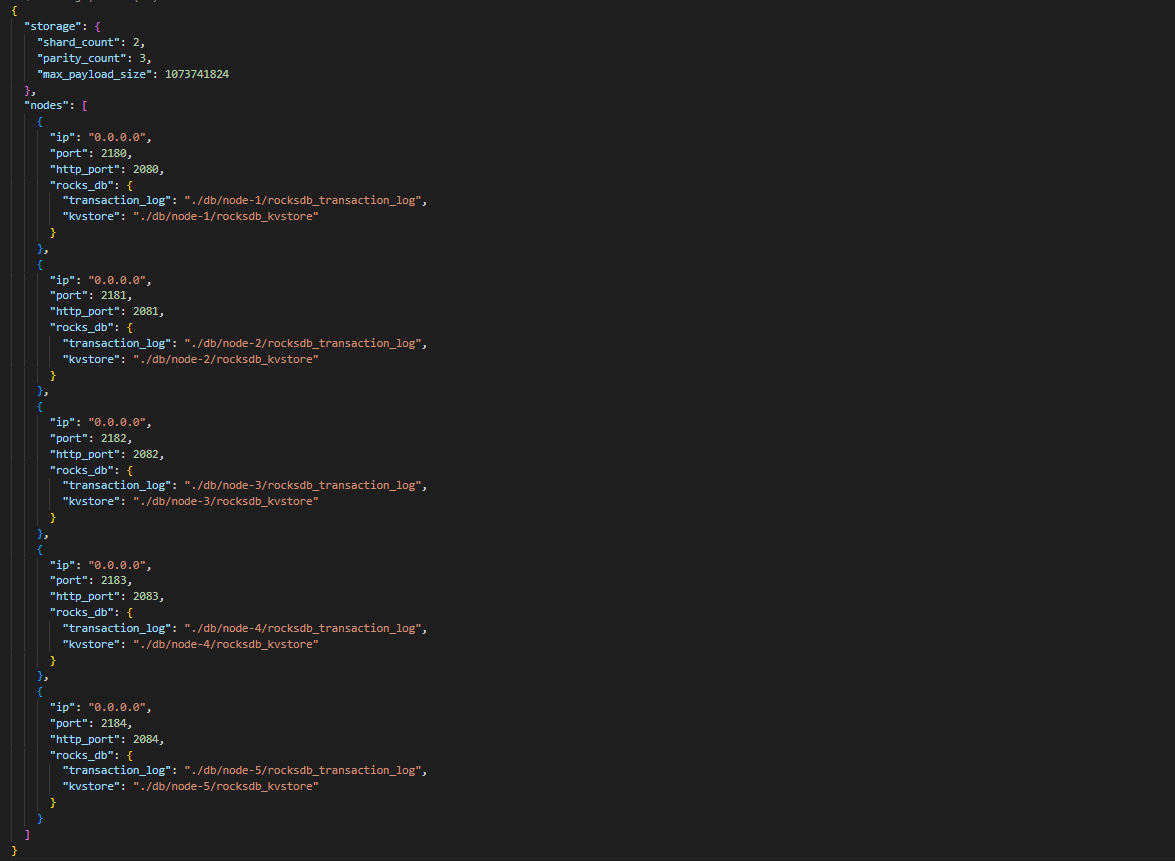
\includegraphics[width=0.80\textwidth]{resources/chapter-4/konfigurasi.png}
	\caption{File konfigurasi yang digunakan}
	\label{fig:config-json}
\end{figure}

Untuk masing-masing node, konfigurasi yang ada adalah \textit{ip}, \textit{port}, \textit{port http}, \textit{path} untuk \textit{transaction log}, dan \textit{path} untuk data persisten \textit{key-value store database}. Konfigurasi global yang ada selain konfigurasi masing-masing node adalah \textit{storage}, yaitu jumlah \textit{data shard} dan \textit{parity shard} untuk erasure coding serta ukuran \textit{payload} maksimal yang akan diterima sistem. File konfigurasi yang digunakan dapat dilihat pada Gambar \ref{fig:config-json}.

Pengaturan sistem untuk menggunakan \textit{erasure coding} atau replikasi tidak terdapat pada file konfigurasi sistem, namun dilakukan saat menjalankan sistem. Pengguna dapat memilih untuk menggunakan \textit{erasure coding} atau
replikasi dengan menggunakan \textit{flag}. Dengan demikian, konfigurasi yang digunakan untuk \textit{erasure coding} dan replikasi adalah sama. Untuk replikasi, jumlah \textit{data shard} dan \textit{parity shard} akan diabaikan dan jumlah keduanya akan dianggap sebagai jumlah \textit{node} secara keseluruhan.

Setup dari sistem dilakukan dengan menjalankan perintah pada file scripts.sh yang sudah disebutkan pada Bagian \ref{subsubsection:implementasi-benchmark}, yaitu run\_all. Perintah ini akan menjalankan semua \textit{node} dari sistem \textit{key-value store database} sesuai dengan konfigurasi pada file ./etc/config.json. Pada dasarnya, run\_all akan menghapus data persisten dan log dari semu \textit{node} yang ada, agar sistem tidak melakukan hal ini, dapat digunakan flag --continue.

Fitur \textit{erasure coding} diaktifkan dengan menambahkan \textit{flag} --erasure. Selain itu, \textit{flag} --trace dapat digunakan untuk mengaktifkan \textit{tracing} pada sistem. Pengaktifan \textit{tracing} akan menghasilkan log yang dapat digunakan untuk analisis lebih lanjut. Pengeluaran \textit{log} ke file dapat dilakukan dengan menambahkan \textit{flag} --file\_output. Penambahan \textit{flag} ini akan mengeluarkan output dari proses ke folder \textit{logs} dalam file bernama node\_(address)\_(port).log.
\subsection{Pengujian sistem}
\label{subsection:pengujian-sistem}

Pengujian sistem dilakukan untuk memastikan bahwa sistem yang telah diimplementasikan berfungsi sesuai dengan yang diharapkan. Kebutuhan dari sistem dapat dilihat pada Bagian \ref{tab:functional-requirements} dan Bagian \ref{tab:non-functional-requirements}. Pengujian akan merujuk pada kebutuhan fungsional dan non-fungsional untuk spesifikasi perilaku sistem yang diharapkan. Untuk memudahkan pemetaan dan memastikan semua pengujian telah mencakup semua kebutuhan, Lampiran \ref{appendix:pemetaan-pengujian} menyediakan tabel yang memetakan kebutuhan fungsional dan non-fungsional ke pengujian yang dilakukan.

\subsubsection{Pengujian operasi dasar}
\label{subsubsection:pengujian-operasi-dasar}

Pengujian ini mencakup fungsional F-1, yaitu bahwa sistem harus dapat melakukan operasi \textit{read} dan \textit{write} pada sebuah \textit{key-value store database}. Pengujian dibagi dua menjadi pengujian operasi \textit{write} dan \textit{read}. Kode dari pengujian tersebut adalah P-1 dan P-2. Pengujian ini menggunakan \textit{script} pembantu oneshot.js yang sudah dijelaskan pada Bagian \ref{subsubsection:implementasi-benchmark}.

Pengujian operasi \textit{write} dengan kode pengujian P-1 dilakukan dengan skenario pengguna menuliskan \textit{key-value pair} ke dalam sistem. Nilai \textit{key} dan \textit{value} akan bersifat acak. Berikut langkah-langkah yang dilakukan dalam pengujian ini:

\begin{enumerate}
	\item Menunggu hingga sistem siap menerima \textit{request}. Konfirmasi dapat dilakukan dengan mengirim \textit{request} HTTP pada \textit{endpoint} /status dan memastikan bahwa sistem sudah memiliki \textit{leader}.
	\item Menjalankan \textit{script} oneshot.js dengan argumen \textit{write} untuk melakukan pengujian operasi dasar. \textit{Script} ini akan mengirimkan \textit{request} \textit{write} ke sistem.
	\item Mengirim request HTTP pada \textit{endpoint} /log untuk memastikan bahwa sistem telah menerima \textit{request} \textit{write} dan telah menyimpan data yang dituliskan.
	\item Mengulangi pengujian dengan sistem \textit{erasure coding} dan juga dengan sistem replikasi.
\end{enumerate}

Hasil yang diharapkan setelah tes dijalankan adalah sistem menyimpan \textit{log} yang berisi \textit{key-value pair} yang telah dituliskan. Untuk \textit{erasure coding}, log yang disimpan harus berisi \textit{key-value pair} yang telah di-\textit{encode} sesuai dengan konfigurasi serta berbeda-beda untuk setiap \textit{node} sesuai dengan index \textit{fragment} yang diterima.

Pengujian operasi \textit{read} dengan kode pengujian P-2 dilakukan dengan skenario pengguna membaca \textit{key-value pair} yang sudah dituliskan sebelumnya. Berikut langkah-langkah yang dilakukan dalam pengujian ini:

\begin{enumerate}
	\item Menunggu hingga sistem siap menerima \textit{request}. Konfirmasi dapat dilakukan dengan mengirim \textit{request} HTTP pada \textit{endpoint} /status dan memastikan bahwa sistem sudah memiliki \textit{leader}.
	\item Menjalankan \textit{script} oneshot.js dengan argumen \textit{read} untuk melakukan pengujian operasi dasar. \textit{Script} ini akan mengirimkan \textit{request} \textit{read} ke sistem.
	\item Mengirim request HTTP pada \textit{endpoint} /log untuk memastikan bahwa sistem mengembalikan nilai \textit{request} \textit{read} yang sesuai dengan nilai yang disimpan pada \textit{log}.
	\item Mengulangi pengujian dengan sistem \textit{erasure coding} dan juga dengan sistem replikasi.
\end{enumerate}

Hasil yang diharapkan setelah tes dijalankan adalah sistem mengembalikan nilai \textit{key-value pair} yang telah dituliskan sebelumnya. Untuk \textit{erasure coding}, sistem harus dapat mengembalikan nilai \textit{key-value pair} yang utuh dan bukan nilai \textit{fragment} yang di-\textit{encode}.
\subsubsection{Pengujian penyimpanan data persistent}
\label{subsubsection:pengujian-penyimpanan-data-persistent}

Pengujian ini mencakup fungsional F-2, yaitu bahwa sistem harus dapat menyimpan data secara persistent pada \textit{key-value store database}. Pengujian dilakukan dengan kode pengujian P-3. Pengujian ini menggunakan \textit{script} pembantu oneshot.js yang sudah dijelaskan pada bagian \ref{subsubsection:implementasi-benchmark}.

Pengujian penyimpanan data \textit{persistent} dengan kode pengujian P-3 dilakukan dengan menuliskan \textit{key-value pair} ke dalam sistem, kemudian mematikan sistem, menyalakan kembali sistem dengan flag --continue, dan memastikan bahwa data yang dituliskan sebelumnya masih dapat diterima. Berikut langkah-langkah yang dilakukan dalam pengujian ini:

\begin{enumerate}
  \item Menunggu hingga sistem siap menerima \textit{request}. Konfirmasi dapat dilakukan dengan mengirim \textit{request} HTTP pada \textit{endpoint} /status dan memastikan bahwa sistem sudah memiliki \textit{leader}.
  \item Menjalankan \textit{script} oneshot.js dengan argumen \textit{write} untuk melakukan pengujian operasi dasar. \textit{Script} ini akan mengirimkan \textit{request} \textit{write} ke sistem.
  \item Mengirim request HTTP pada \textit{endpoint} /log untuk memastikan bahwa sistem telah menerima \textit{request} \textit{write} dan telah menyimpan data yang dituliskan.
  \item Mematikan sistem dengan menggunakan perintah stop\_all pada file scripts.sh.
  \item Menyalakan ulang sistem dengan menggunakan perintah run\_all pada file scripts.sh dengan tambahan flag --continue. Flag ini akan membuat sistem tidak menghapus data persisten yang sudah ada sebelumnya.
  \item Menjalankan \textit{script} oneshot.js dengan argumen \textit{read} untuk melakukan pengujian operasi dasar. \textit{Script} ini akan mengirimkan \textit{request} \textit{read} ke sistem.
  \item Mengirim request HTTP pada \textit{endpoint} /log untuk memastikan bahwa sistem mengembalikan nilai \textit{request} \textit{read} yang sesuai dengan nilai yang disimpan pada \textit{log}.
  \item Mengulangi pengujian dengan sistem \textit{erasure coding} dan juga dengan sistem replikasi.
\end{enumerate}

Hasil yang diharapkan setelah tes dijalankan adalah sistem mengembalikan nilai \textit{key-value pair} yang telah dituliskan sebelumnya. Untuk \textit{erasure coding}, sistem harus dapat mengembalikan nilai \textit{key-value pair} yang utuh dan bukan nilai \textit{fragment} yang di-\textit{encode}. Pengujian ini memastikan bahwa data yang disimpan pada sistem tetap ada meskipun sistem dimatikan dan dinyalakan kembali.
\subsubsection{Pengujian pencatatan waktu transaksi}
\label{subsubsection:pengujian-pencatatan-waktu-transaksi}

Pengujian ini mencakup fungsional F-3, yaitu bahwa sistem harus dapat mencatat waktu transaksi dari \textit{request} masuk hingga operasi selesai. Pengujian dibagi dua menjadi pengujian pencatatan waktu transaksi untuk operasi \textit{write} dan operasi \textit{read}. Kode dari pengujian tersebut adalah P-4 dan P-5. Pengujian ini menggunakan \textit{script} pembantu oneshot.js yang sudah dijelaskan pada bagian \ref{subsubsection:implementasi-benchmark}.

Pengujian pencatatan waktu transaksi dengan kode pengujian P-4 dilakukan dengan skenario pengguna mengirimkan \textit{request} \textit{write} ke sistem. Pengujian dilakukan dengan langkah-langkah sebagai berikut:

\begin{enumerate}
  \item Melakukan setup sistem menggunakan \textit{flag} --trace dan --file\_output seperti yang dijelaskan pada bagian \ref{subsection:setup-pengujian}.
  \item Menunggu hingga sistem siap menerima \textit{request}. Konfirmasi dapat dilakukan dengan mengirim \textit{request} HTTP pada \textit{endpoint} /status dan memastikan bahwa sistem sudah memiliki \textit{leader}.
  \item Menjalankan \textit{script} oneshot.js dengan argumen \textit{write} untuk melakukan pengujian operasi dasar. \textit{Script} ini akan mengirimkan \textit{request} \textit{write} ke sistem.
  \item Mengecek \textit{log} yang dihasilkan oleh sistem pada file \textit{output log} dan memastikan bahwa sistem mencatat waktu transaksi.
  \item Mengulangi pengujian dengan sistem \textit{erasure coding} dan juga dengan sistem replikasi.
\end{enumerate}

Hasil yang diharapkan adalah sistem menghasilkan \textit{log} yang memiliki informasi waktu setiap fungsi yang dipanggil dalam sebuah \textit{request} dari masuk hingga selesai. Contoh bentuk \textit{log} yang dihasilkan dapat dilihat pada gambar \ref{fig:log-trace}.

\begin{figure}[ht]
    \centering
    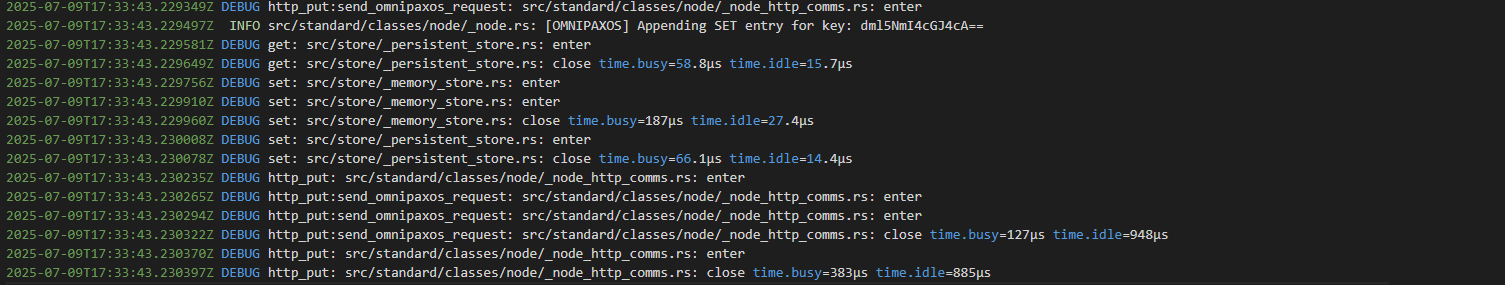
\includegraphics[width=0.95\textwidth]{resources/chapter-4/log-trace.png}
    \caption{Contoh log yang dihasilkan oleh sistem}
    \label{fig:log-trace}
\end{figure}

Pengujian pencatatan waktu transaksi dengan kode pengujian P-5 dilakukan dengan skenario pengguna mengirimkan \textit{request} \textit{read} ke sistem. Pengujian dilakukan dengan langkah-langkah sebagai berikut:

\begin{enumerate}
  \item Melakukan setup sistem menggunakan \textit{flag} --trace dan --file\_output seperti yang dijelaskan pada bagian \ref{subsection:setup-pengujian}.
  \item Menunggu hingga sistem siap menerima \textit{request}. Konfirmasi dapat dilakukan dengan mengirim \textit{request} HTTP pada \textit{endpoint} /status dan memastikan bahwa sistem sudah memiliki \textit{leader}.
  \item Menjalankan \textit{script} oneshot.js dengan argumen \textit{read} untuk melakukan pengujian operasi dasar. \textit{Script} ini akan mengirimkan \textit{request} \textit{read} ke sistem.
  \item Mengecek \textit{log} yang dihasilkan oleh sistem pada file \textit{output log} dan memastikan bahwa sistem mencatat waktu transaksi.
  \item Mengulangi pengujian dengan sistem \textit{erasure coding} dan juga dengan sistem replikasi.
\end{enumerate}

Hasil yang diharapkan adalah sistem menghasilkan \textit{log} yang memiliki informasi waktu setiap fungsi yang dipanggil dalam sebuah \textit{request} dari masuk hingga selesai. Contoh bentuk \textit{log} yang dihasilkan mirip dengan gambar \ref{fig:log-trace} dengan perbedaan pada \textit{request} yang dikirim adalah \textit{read}.
\subsubsection{Pengujian encoding data menggunakan erasure coding}
\label{subsubsection:pengujian-encoding-data-erasure-coding}

\subsubsection{Pengujian rekonstruksi data}
\label{subsubsection:pengujian-rekonstruksi-data}

Pengujian ini mencakup fungsional F-5, yaitu bahwa sistem harus dapat merekonstruksi data dari data yang disimpan menggunakan \textit{erasure coding}. Pengujian dilakukan dengan kode pengujian P-7. Pengujian ini menggunakan \textit{script} pembantu oneshot.js yang sudah dijelaskan pada bagian \ref{subsubsection:implementasi-benchmark}. Pengujian ini dilakukan dengan menuliskan \textit{key-value pair} ke dalam sistem lalu melakukan operasi \textit{read} pada \textit{key-value pair} tersebut untuk memastikan bahwa data yang disimpan telah di-\textit{encode} sesuai dengan konfigurasi yang telah ditentukan dan dapat direkonstruksi.

Pengujian rekonstruksi data dengan kode pengujian P-7 dilakukan dengan langkah-langkah sebagai berikut:
\begin{enumerate}
  \item Menunggu hingga sistem siap menerima \textit{request}. Konfirmasi dapat dilakukan dengan mengirim \textit{request} HTTP pada \textit{endpoint} /status dan memastikan bahwa sistem sudah memiliki \textit{leader}.
  \item Menjalankan \textit{script} oneshot.js dengan argumen \textit{write} untuk melakukan pengujian operasi dasar. \textit{Script} ini akan mengirimkan \textit{request} \textit{write} ke sistem.
  \item Mengirim \textit{request} HTTP pada \textit{endpoint} /fragment untuk memastikan bahwa sistem telah menerima \textit{request} \textit{write} dan telah menyimpan data yang dituliskan dalam bentuk \textit{fragment} yang telah di-\textit{encode}.
  \item Mengirim \textit{request} HTTP pada \textit{endpoint} /read untuk memastikan bahwa sistem dapat mengembalikan nilai \textit{key-value pair} yang telah di-\textit{encode} sesuai dengan konfigurasi yang telah ditentukan.
\end{enumerate}

Hasil yang diharapkan setelah tes dijalankan adalah sistem mengembalikan nilai \textit{key-value pair} yang telah dituliskan sebelumnya. Sistem harus dapat mengembalikan nilai \textit{key-value pair} yang utuh dan bukan nilai \textit{fragment} yang di-\textit{encode}.

Selain pengujian yang dilakukan dengan kode P-7, pengujian untuk kebutuhan fungsional F-4 juga dilakukan dengan \textit{automated testing} pada \textit{test suite} repository OmniPaxos. Pengujian yang dilakukan pada \textit{test suite} tersebut mengetes implementasi \textit{Erasure Coding Service} yang dibuat terlepas dari sistem \textit{key-value store database}.
\subsubsection{Pengujian distribusi data}
\label{subsubsection:pengujian-distribusi-data}

Pengujian ini mencakup fungsional F-5, yaitu bahwa sistem harus dapat mendistribusikan data atau sebagian data ke \textit{node} lain untuk keperluan ketahanan data. Pengujian dilakukan dengan kode pengujian P-8. Pengujian ini menggunakan \textit{script} pembantu oneshot.js yang sudah dijelaskan pada bagian \ref{subsubsection:implementasi-benchmark}. Pengujian ini dilakukan dengan menuliskan \textit{key-value pair} ke dalam sistem. Setelah itu, dilakukan melakukan \textit{request} GET ke \textit{endpoint} /fragment ke beberapa node lain untuk sistem \textit{erasure coding} dan \textit{endpoint} /read untuk sistem replikasi. Hal ini untuk memastikan bahwa data yang disimpan telah didistribusikan ke \textit{node} lain sesuai dengan konfigurasi yang telah ditentukan.

Pengujian distribusi data dengan kode pengujian P-8 dilakukan dengan langkah-langkah sebagai berikut:
\begin{enumerate}
    \item Menunggu hingga sistem siap menerima \textit{request}. Konfirmasi dapat dilakukan dengan mengirim \textit{request} HTTP pada \textit{endpoint} /status dan memastikan bahwa sistem sudah memiliki \textit{leader}.
    \item Menjalankan \textit{script} oneshot.js dengan argumen \textit{write} untuk melakukan pengujian operasi dasar. \textit{Script} ini akan mengirimkan \textit{request} \textit{write} ke sistem.
    \item Mengirim \textit{request} HTTP pada \textit{endpoint} /fragment ke beberapa \textit{node} lain untuk memastikan bahwa sistem telah mendistribusikan data yang dituliskan dalam bentuk \textit{fragment} yang telah di-\textit{encode}. Untuk sistem replikasi, mengirim \textit{request} HTTP pada \textit{endpoint} /read ke beberapa \textit{node} lain untuk memastikan bahwa sistem telah mendistribusikan data yang dituliskan ke \textit{node} lain.
    \item Mengirim \textit{request} HTTP pada \textit{endpoint} /read untuk memastikan bahwa sistem dapat mengembalikan nilai \textit{key-value pair} yang telah didistribusikan ke \textit{node} lain.
\end{enumerate}

Hasil yang diharapkan setelah tes dijalankan adalah sistem mengembalikan nilai \textit{key-value pair} yang telah didistribusikan. Untuk sistem \textit{erasure coding}, sistem harus dapat mengembalikan nilai \textit{key-value pair} yang berbentuk \textit{fragment} ter-\textit{encode}. Untuk sistem replikasi, sistem harus dapat mengembalikan nilai \textit{key-value pair} yang utuh.
\subsubsection{Pengujian konfigurasi sistem}
\label{subsubsection:pengujian-konfigurasi-sistem}

Pengujian ini mencakup fungsional F-7, yaitu bahwa sistem harus dapat dikonfigurasi untuk menggunakan \textit{erasure coding} atau replikasi tanpa mengganti konfigurasi lainnya. Pengujian dilakukan dengan kode pengujian P-9. Pengujian ini mencakup proses menjalankan sistem dengan konfigurasi yang sama dengan \textit{flag} tambahan --erasure dan tanpa \textit{flag} tersebut seperti yang sudah dijelaskan pada bagian \ref{subsection:setup-pengujian}.

Pengujian konfigurasi sistem dengan kode pengujian P-9 dilakukan dengan langkah-langkah sebagai berikut:
\begin{enumerate}
  \item Menyalakan sistem dengan konfigurasi \textit{erasure coding} menggunakan \textit{flag} --erasure. Konfirmasi dapat dilakukan dengan mengirim \textit{request} HTTP pada \textit{endpoint} /status dan memastikan bahwa sistem sudah memiliki \textit{leader}.
  \item Mematikan sistem dengan menggunakan perintah stop\_all pada file scripts.sh.
  \item Menyalakan ulang sistem tanpa \textit{flag} --erasure. Konfirmasi dapat dilakukan dengan mengirim \textit{request} HTTP pada \textit{endpoint} /status dan memastikan bahwa sistem sudah memiliki \textit{leader}.
\end{enumerate}

Hasil yang diharapkan setelah tes dijalankan adalah sistem dapat berjalan dengan konfigurasi \textit{erasure coding} dan juga dapat berjalan tanpa \textit{flag} tersebut. Tujuannya adalah untuk memastikan bahwa sistem dapat berjalan dengan konfigurasi yang sama dan hanya berbeda pada penggunaan \textit{erasure coding} atau replikasi.
\subsubsection{Pengujian perubahan konfigurasi ketahanan sistem}
\label{subsubsection:pengujian-perubahan-konfigurasi-ketahanan}

Pengujian ini mencakup fungsional F-8, yaitu bahwa sistem harus dapat mengubah konfigurasi ketahanan sistem tanpa mempengaruhi operasi lainnya. Pengujian dilakukan dengan kode pengujian P-10.

Pengujian perubahan konfigurasi ketahanan sistem dengan kode pengujian P-10 mencakup proses mengubah konfigurasi sistem dengan jumlah \textit{data shard} dan \textit{parity shard} yang berbeda-beda. Pengujian ini dilakukan dengan mengubah konfigurasi sistem pada file config.json yang sudah dijelaskan pada Bagian \ref{subsection:setup-pengujian}. Berikut langkah-langkah yang dilakukan dalam pengujian ini:

\begin{enumerate}
	\item Mengubah konfigurasi sistem pada file config.json dengan jumlah \textit{data shard} dan \textit{parity shard} yang berbeda.
	\item Menyalakan ulang sistem untuk menerapkan perubahan konfigurasi. Konfirmasi dapat dilakukan dengan mengirim \textit{request} HTTP pada \textit{endpoint} /status dan memastikan bahwa sistem sudah memiliki \textit{leader}.
	\item Melakukan pengujian operasi \textit{write} dan \textit{read} untuk memastikan bahwa sistem masih berfungsi dengan baik setelah perubahan konfigurasi.
\end{enumerate}

Hasil yang diharapkan setelah tes dijalankan adalah sistem dapat berfungsi dengan baik setelah perubahan konfigurasi. Sistem harus dapat menyimpan dan mengambil data dengan jumlah \textit{data shard} dan \textit{parity shard}.
\subsubsection{Pengujian Request dengan Ukuran Data bervariasi}
\label{subsubsection:pengujian-request-ukuran-data}

Pengujian ini mencakup fungsional F-9, yaitu bahwa sistem harus dapat mensimulasikan \textit{request} dengan ukuran data yang bervariasi. Pengujian ini dilakukan dengan kode pengujian P-11.

Pengujian request dengan ukuran data bervariasi dengan kode pengujian P-11 dilakukan melalui mengatur variabel \textit{size} dan menjalankan perintah run\_bench\_suite pada file scripts.sh yang sudah dijelaskan pada bagian \ref{subsection:setup-pengujian}. Berikut langkah-langkah yang dilakukan dalam pengujian ini:

\begin{enumerate}
    \item Menunggu hingga sistem siap menerima \textit{request}. Konfirmasi dapat dilakukan dengan mengirim \textit{request} HTTP pada \textit{endpoint} /status dan memastikan bahwa sistem sudah memiliki \textit{leader}.
    \item Mengatur variabel \textit{size} pada file scripts.js dengan ukuran data yang bervariasi. Variabel ini menentukan seberapa besar data yang akan disimpan dalam sistem.
    \item Menjalankan perintah run\_bench\_suite pada file scripts.sh untuk menjalankan pengujian dengan ukuran data yang telah ditentukan.
\end{enumerate}

Hasil yang diharapkan setelah tes dijalankan adalah sistem dapat memulai \textit{benchmark} dengan \textit{request} dengan ukuran data yang bervariasi secara otomatis. Perlu dipastikan juga dalam penjalanan run\_bench\_suite tidak terdapat balikan \textit{error} dari sistem.
\subsubsection{Pengujian pengumpulan data}
\label{subsubsection:pengujian-pengumpulan-data}

Pengujian ini mencakup fungsional F-10, yaitu bahwa sistem harus dapat menjalankan \textit{request} secara berulang kali dan bervariasi secara otomatis untuk pengumpulan data. Pengujian dilakukan dengan kode pengujian P-12. Pengujian dilakukan dengan menjalankan perintah run\_bench\_suite pada file scripts.sh yang sudah dijelaskan pada bagian \ref{subsection:setup-pengujian}. Setelah itu dilakukan verifikasi dari durasi \textit{benchmark} yang dilakukan bahwa sistem menerima \textit{request} secara berulang kali.

Pengujian pengumpulan data dengan kode pengujian P-12 dilakukan dengan langkah-langkah sebagai berikut:
\begin{enumerate}
    \item Menunggu hingga sistem siap menerima \textit{request}. Konfirmasi dapat dilakukan dengan mengirim \textit{request} HTTP pada \textit{endpoint} /status dan memastikan bahwa sistem sudah memiliki \textit{leader}.
    \item Menjalankan perintah run\_bench\_suite pada file scripts.sh.
    \item Memastikan bahwa sistem menerima \textit{request} secara berulang kali. Hal ini dapat dilakukan dengan melihat \textit{log} dari sistem dan hasil laporan yang dibuat oleh k6.
\end{enumerate}

Hasil yang diharapkan setelah tes dijalankan adalah sistem dapat menjalankan \textit{request} secara berulang kali secara otomatis, yaitu dalam satu \textit{benchmark}, sistem tidak hanya menerima satu \textit{request} saja. Perlu dipastikan juga dalam penjalanan run\_bench\_suite tidak terdapat balikan \textit{error} dari sistem.
\subsubsection{Pengujian consistency}
\label{subsubsection:pengujian-consistency}

Pengujian ini mencakup non-fungsional NF-1, yaitu bahwa sistem harus menyediakan \textit{consistency} yang tinggi dengan \textit{request} ke \textit{node} manapun harus menghasilkan hasil yang sama. Pengujian dilakukan dengan kode pengujian P-12. Disebabkan kebutuhan ini merupakan non-fungsional dan sulit untuk diuji secara langsung, maka pengujian dilakukan dengan mendekati kebutuhan ini. Pengujian dilakukan dengan menjalankan operasi \textit{write} dan \textit{read} dengan hampir bersamaan pada beberapa \textit{node} yang berbeda. Pengujian ini dilakukan dengan memanfaatkan \textit{script} oneshot.js yang sudah dijelaskan pada bagian \ref{subsubsection:implementasi-benchmark}.

Pengujian consistency dengan kode pengujian P-13 dilakukan dengan langkah-langkah sebagai berikut:
\begin{enumerate}
    \item Menunggu hingga sistem siap menerima \textit{request}. Konfirmasi dapat dilakukan dengan mengirim \textit{request} HTTP pada \textit{endpoint} /status dan memastikan bahwa sistem sudah memiliki \textit{leader}.
    \item Secara bersamaan, menjalankan \textit{script} oneshot.js dengan argumen \textit{write} dan \textit{read} pada beberapa \textit{node} yang berbeda. Hal ini dilakukan untuk mensimulasikan \textit{request} yang hampir bersamaan ke beberapa \textit{node}.
    \item Mengirim \textit{request} HTTP pada \textit{endpoint} /log untuk memastikan bahwa sistem telah menerima \textit{request} \textit{write} dan telah menyimpan data yang dituliskan.
    \item Mengulangi pengujian dengan sistem \textit{erasure coding} dan juga dengan sistem replikasi.
\end{enumerate}

Hasil yang diharapkan adalah sistem tidak mengembalikan nilai hingga \textit{request} \textit{write} selesai. Selain itu, setiap \textit{node} pada sistem harus mengembalikan nilai \textit{key-value pair} yang sama pada operasi \textit{read}.

\subsubsection{Pengujian availability}
\label{subsubsection:pengujian-availability}

Pengujian ini mencakup non-fungsional NF-2, yaitu bahwa sistem harus memiliki \textit{availability} yang tinggi dengan harus dapat tetap tersedia walaupun beberapa \textit{node} ada dalam kondisi gagal. Pengujian dilakukan dengan kode pengujian P-14.

Pengujian availability dengan kode pengujian P-14 dilakukan dengan menjalankan sistem, melakukan operasi \textit{write}, mematikan beberapa \textit{node}, dan melakukan operasi \textit{read} dengan beberapa \textit{node} dalam kondisi mati. Pengujian ini dilakukan dengan memanfaatkan \textit{script} oneshot.js yang sudah dijelaskan pada Bagian \ref{subsubsection:implementasi-benchmark}. Berikut langkah-langkah yang dilakukan dalam pengujian ini:

\begin{enumerate}
	\item Menunggu hingga sistem siap menerima \textit{request}. Konfirmasi dapat dilakukan dengan mengirim \textit{request} HTTP pada \textit{endpoint} /status dan memastikan bahwa sistem sudah memiliki \textit{leader}.
	\item Menjalankan \textit{script} oneshot.js dengan argumen \textit{write} untuk melakukan pengujian operasi dasar. \textit{Script} ini akan mengirimkan \textit{request} \textit{write} ke sistem.
	\item Mengirim \textit{request} HTTP pada \textit{endpoint} /log untuk memastikan bahwa sistem telah menerima \textit{request} \textit{write} dan telah menyimpan data yang dituliskan.
	\item Mematikan beberapa \textit{node} dengan masuk ke GNU screen tempat proses tersebut berjalan dan mengirimkan SIGTERM ke proses tersebut.
	\item Menjalankan \textit{script} oneshot.js dengan argumen \textit{read} untuk melakukan pengujian operasi dasar. \textit{Script} ini akan mengirimkan \textit{request} \textit{read} ke sistem.
	\item Mengirim \textit{request} HTTP pada \textit{endpoint} /log untuk memastikan bahwa sistem mengembalikan nilai \textit{request} \textit{read} yang sesuai dengan nilai yang disimpan pada \textit{log}.
	\item Mengulangi pengujian dengan sistem \textit{erasure coding} dan juga dengan sistem replikasi.
\end{enumerate}

Hasil yang diharapkan setelah tes dijalankan adalah sistem mengembalikan nilai \textit{key-value pair} yang telah dituliskan sebelumnya meskipun beberapa \textit{node} dalam kondisi mati. Untuk sistem \textit{erasure coding}, sistem harus dapat mengembalikan nilai \textit{key-value pair} yang utuh dan bukan nilai \textit{fragment} yang di-\textit{encode}. Pengujian ini memastikan bahwa sistem tetap tersedia meskipun beberapa \textit{node} mengalami kegagalan.
\subsubsection{Pengujian penyimpanan minimal}
\label{subsubsection:pengujian-penyimpanan-minimal}

Pengujian ini mencakup non-fungsional NF-3, yaitu bahwa sistem harus menggunakan penyimpanan minimal untuk skalabilitas dan efisiensi biaya. Pengujian dilakukan dengan kode pengujian P-15. Disebabkan kebutuhan ini sulit untuk diuji secara langsung, pengujian ini hanya mencakup memperlihatkan jumlah penyimpanan yang digunakan oleh sistem.

Pengujian penyimpanan minimal dengan kode pengujian P-15 dilakukan dengan melakukan operasi \textit{write} lalu melihat data yang disimpan pada sistem. Berikut langkah-langkah yang dilakukan dalam pengujian ini:

\begin{enumerate}
	\item Menunggu hingga sistem siap menerima \textit{request}. Konfirmasi dapat dilakukan dengan mengirim \textit{request} HTTP pada \textit{endpoint} /status dan memastikan bahwa sistem sudah memiliki \textit{leader}.
	\item Mengirim \textit{request} HTTP pada \textit{endpoint} /write untuk menyimpan data ke dalam sistem. Data yang disimpan dapat berupa \textit{key-value pair} yang berisi informasi yang relevan untuk pengujian.
	\item Mengirim \textit{request} HTTP pada \textit{endpoint} /log untuk memastikan bahwa sistem telah menerima \textit{request} \textit{write} dan telah menyimpan data yang dituliskan.
	\item Memeriksa ukuran penyimpanan yang digunakan oleh sistem.
	\item Mengulangi pengujian dengan sistem \textit{erasure coding} dan juga dengan sistem replikasi.
\end{enumerate}

Hasil yang diharapkan setelah tes dijalankan adalah sistem dapat menyimpan data dengan ukuran penyimpanan yang minimal. Untuk \textit{erasure coding}, log yang disimpan harus berisi \textit{key-value pair} yang telah di-\textit{encode} sesuai dengan konfigurasi.
\subsubsection{Pengujian response time rendah}
\label{subsubsection:pengujian-response-time-rendah}

Pengujian ini mencakup non-fungsional NF-5, yaitu bahwa sistem harus dapat memberikan \textit{response time} yang rendah untuk operasi \textit{write} dan \textit{read}. Pengujian dilakukan dengan kode pengujian P-16. Disebabkan kebutuhan ini sulit untuk diuji secara langsung, maka pengujian ini hanya mencakup memperlihatkan kinerja \textit{response time} sistem.


Pengujian \textit{response time} minimal dengan kode pengujian P-16 dilakukan dengan menjalankan perintah run\_bench\_suite pada file scripts.sh yang sudah dijelaskan pada Bagian \ref{subsection:setup-pengujian}. Berikut langkah-langkah yang dilakukan dalam pengujian ini:

\begin{enumerate}
  \item Menunggu hingga sistem siap menerima \textit{request}. Konfirmasi dapat dilakukan dengan mengirim \textit{request} HTTP pada \textit{endpoint} /status dan memastikan bahwa sistem sudah memiliki \textit{leader}.
  \item Menjalankan perintah run\_bench\_suite pada file scripts.sh untuk menjalankan pengujian \textit{response time} dengan ukuran data yang telah ditentukan.
  \item Mengulangi pengujian dengan sistem \textit{erasure coding} dan juga dengan sistem replikasi.
\end{enumerate}

Hasil yang diharapkan setelah tes dijalankan adalah laporan dari k6 dan hasil \textit{trace log} yang dihasilkan oleh sistem. Laporan ini menunjukkan \textit{response time} dari operasi \textit{write} dan \textit{read} yang dilakukan selama pengujian. Perlu dipastikan juga dalam penjalanan run\_bench\_suite tidak terdapat balikan \textit{error} dari sistem.

\subsection{Analisis Benchmark}
\label{subsection:analisis-benchmark}

Analisis \textit{benchmark} dilakukan untuk mengevaluasi kinerja sistem yang telah diimplementasikan. Analisis dilakukan dengan menggunakan data hasil \textit{benchmark} yang telah dibuat dengan sistem pada Bagian \ref{subsubsection:implementasi-benchmark}. Analisis akan dimulai dari analisis operasi \textit{write}, dilanjut dengan analisis operasi \textit{read}, dan diakhiri dengan analisis keseluruhan dari sistem.

\subsubsection{Setup Benchmark}
\label{subsubsection:setup-benchmark}

Pengaturan variabel yang digunakan dalam \textit{benchmark} dilakukan pada file \textit{scripts.js} seperti yang sudah dijelaskan pada bagian \ref{subsubsection:implementasi-benchmark}. Skenario \textit{benchmark} dibagi menjadi tiga dengan mempertimbangkan hipotesis pengaruh variabel yang dinyatakan pada bagian \ref{sec:rumusan-masalah}. Skenario tersebut adalah sebagai berikut:

\begin{enumerate}
  \item Internet cepat dan \textit{payload} kecil
  
  Skenario ini menggambarkan kondisi ekstrim berlawanan dengan hipotesis yang berpihak pada kinerja replikasi. Skenario ini digunakan untuk menguji apakah sistem \textit{erasure coding} masih dapat bersaing dengan sistem replikasi serta melihat keuntungan dari penggunaan replikasi dalam kondisi tersebut. 

  \item Internet rata-rata dan \textit{payload} umum
  
  Skenario ini bertujuan untuk mencari kondisi perbatasan antara kinerja \textit{erasure coding} dan replikasi. Tujuannya adalah untuk mencari poin ketika sistem \textit{erasure coding} mulai mengungguli sistem replikasi ataupun sebaliknya. Skenario ini juga diharapkan dapat memberikan gambaran umum pengaruh variabel-variabel yang ada terhadap kinerja sistem.
  
  \item Internet lambat dan \textit{payload} umum
  
  Skenario ini menggambarkan kondisi ekstrim berlawanan dengan hipotesis yang berpihak pada kinerja \textit{erasure coding}. Skenario ini digunakan untuk menguji apakah sistem replikasi masih dapat bersaing dengan sistem \textit{erasure coding} serta melihat keuntungan dari penggunaan \textit{erasure coding} dalam kondisi tersebut .

\end{enumerate}

Dari skenario-skenario tersebut, diturunkan beberapa variabel yang akan digunakan pada \textit{benchmark}. Menggunakan sistem \textit{benchmark} yang telah dibuat, variabel ini akan dijalankan untuk semua kombinasi yang dapat dibentuk. Variabel-variabel tersebut dapat dilihat pada tabel \ref{tab:variabel-benchmark}.

\begin{table}[ht]
  \centering
  \caption{Variabel yang digunakan pada \textit{benchmark}}
  \label{tab:variabel-benchmark}
  \begin{tabular}{|c|p{6cm}|p{6cm}|}
    \hline
    \textbf{Skenario} & \textbf{Ukuran \textit{Payload}} & \textbf{Bandwidth} \\ \hline
    1 & 1024 B & 10 Gbps \\ \hline
    2 & 200 KB, 400 KB, 600 KB, 800 KB, 1 MB & 10 Mbps, 25 Mbps, 40 Mbps, 55 Mbps, 70 Mbps \\ \hline
    3 & 200 KB, 400 KB, 600 KB, 800 KB, 1 MB & 256 kbps \\ \hline
  \end{tabular}
\end{table}

Terkait ukuran \textit{payload}, nilai yang diambil adalah berdasarkan ukuran \textit{payload} yang umum digunakan pada aplikasi \textit{key-value store} seperti yang dijelaskan pada bagian \ref{sec:key-value-database}. Penambahan linear dilakukan untuk mempermudah analisis data dan mendapatkan pola yang lebih jelas. Selain itu, untuk bandwidth, nilai yang diambil adalah berdasarkan kecepatan internet yang umum digunakan di Indonesia lalu dilakukan penambahan linear dengan alasan yang sama. Nilai-nilai tersebut diambil dari data yang tersedia pada situs Speedtest Global Index\footnote{\url{https://www.speedtest.net/global-index}}.
\subsubsection{Analisis Operasi Write}
\label{subsubsection:analisis-operasi-write}

Analisis kinerja operasi \textit{write} merupakan inti dari penilitian ini, seperti yang sudah dijelaskan pada bagian \ref{sec:rumusan-masalah}. Analisis ini bertujuan untuk memvalidasi bahwa \textit{erasure coding} dapat mengungguli replikasi dalam kondisi tertentu. Analisis kinerja operasi \textit{write} akan dibagi berdasarkan skenario yang sudah disebutkan pada bagian \ref{subsubsection:setup-benchmark}. Setiap skenario akan dianalisis berdasarkan hasil \textit{benchmark} yang telah dilakukan.

\begin{enumerate}
  \item Skenario 1: Internet cepat dan \textit{payload} kecil

  Pada skenario pertama yang dirancang sebagai kondisi ekstrem yang menguntungkan replikasi, hasil \textit{benchmark} menunjukkan bahwa sistem replikasi memiliki \textit{response time} yang lebih rendah dibandingkan sistem berbasis \textit{erasure coding}. Perbedaan kinerja ini dapat dilihat pada gambar \ref{fig:write-smload-fastnet}.

  \begin{figure}[ht]
      \centering
      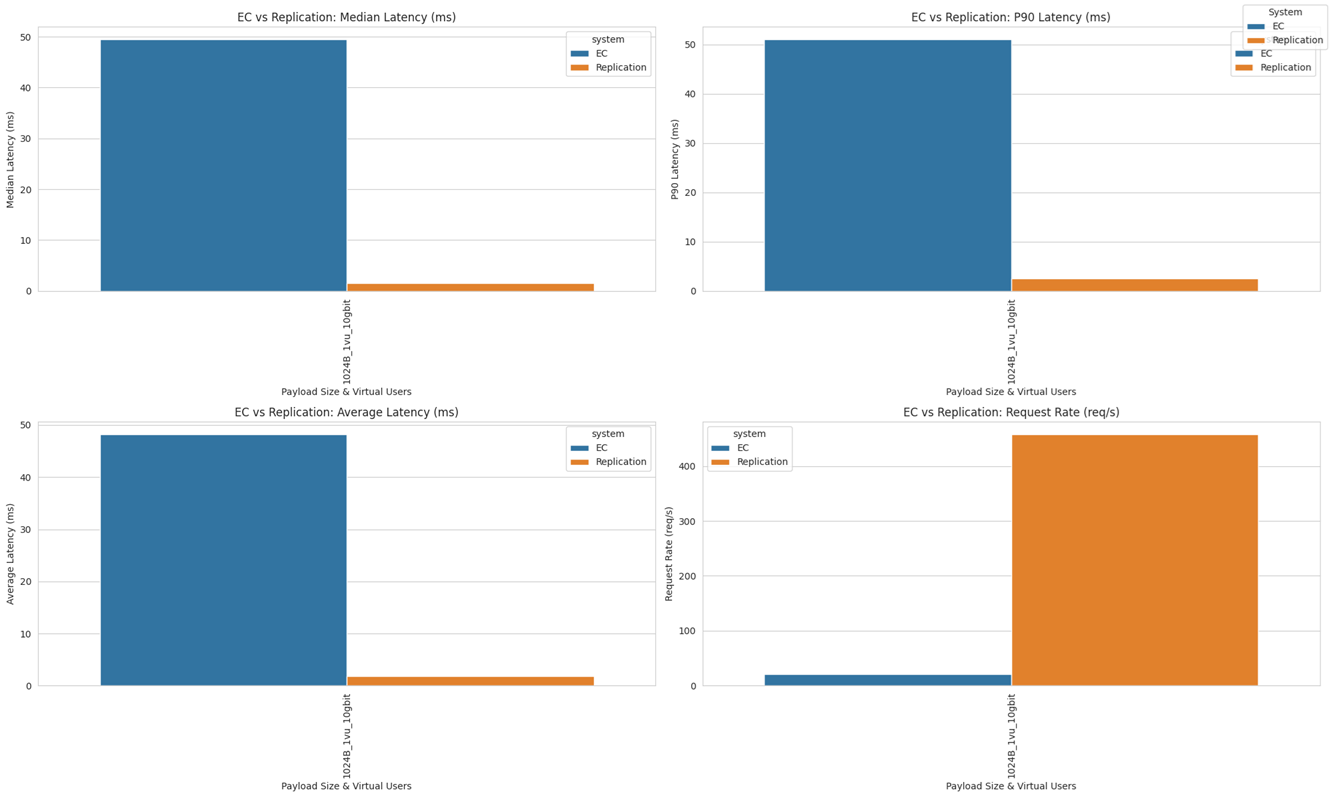
\includegraphics[width=0.8\textwidth]{resources/chapter-4/write_smload_fastnet.png}

      \caption{Kinerja Operasi Write pada Internet Cepat dan Payload Kecil}
      \label{fig:write-smload-fastnet}
  \end{figure}
  
  Interpretasi dari hasil ini terletak pada dinamika komponen latensi. Pada jaringan dengan \textit{bandwidth} tinggi seperti 10 Gbps, waktu yang dibutuhan untuk mentransfer data menjadi kecil. Selain itu, data yang kecil membuat operasi terkait data seperti penulisan pada \textit{memory} dan \textit{disk} menjadi kecil juga. Dengan kecilnya waktu transfer dan operasi terkait data, faktor penentu \textit{response time} adalah biaya komputasi dan \textit{overhead} pemrosesan pada setiap node.

  Dalam skenario ini, proses \textit{erasure coding} yang lebih kompleks membutuhkan waktu yang lebih lama dibandingkan dengan proses replikasi yang lebih sederhana. Lingkungan seperti ini umum ditemukan pada komunikasi antar-\textit{server} dalam satu pusat data modern dengan penggunaan transaksi data berukuran kecil seperti pembaruan metadata, status sesi, atau operasi konfigurasi singkat.
  
  \item Skenario 2: Internet lambat dan \textit{payload} besar
  
  Skenario kedua dirancang sebagai kondisi ekstrem yang berlawanan dengan skenario pertama dengan keuntungan pada \textit{erasure coding}. Hasil \textit{benchmark} pada skenario ini menunjukkan pembalikan kinerja dramatis dengan sistem berbasis \textit{erasure coding} secara konsisten mengungguli replikasi dengan \textit{response time} yang lebih rendah untuk \textit{payload} yang diuji. Gambar \ref{fig:write-bigload-slownet} menunjukkan perbandingan kinerja operasi \textit{write} pada skenario ini.

  \begin{figure}[ht]
      \centering
      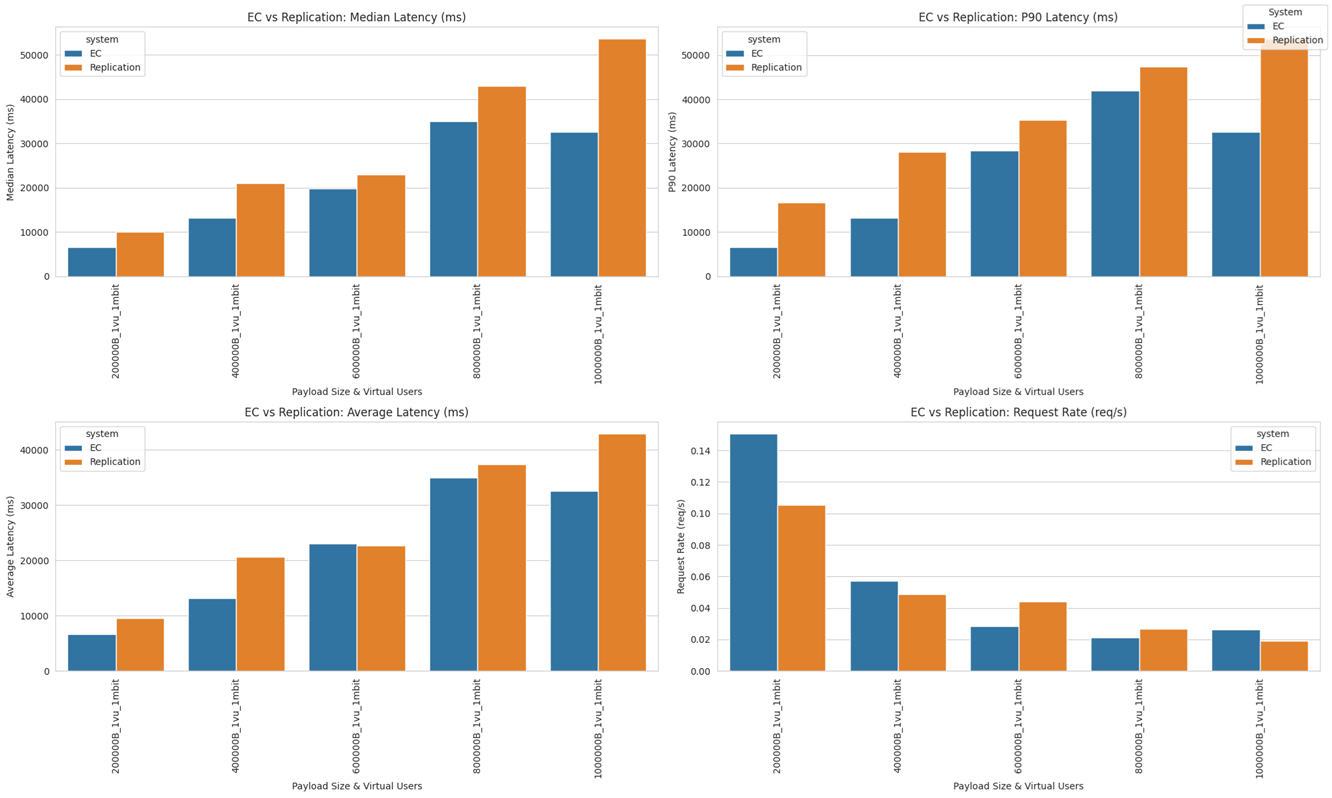
\includegraphics[width=0.8\textwidth]{resources/chapter-4/write_bigload_slownet.png}

      \caption{Kinerja Write pada Internet Lambat dan Payload Besar}
      \label{fig:write-bigload-slownet}
  \end{figure}

  Hasil dari skenario ini mengkonfirmasi bahwa \textit{erasure coding} dapat mengungguli replikasi dalam kondisi tertentu, yaitu dalam skenario dengan \textit{bandwidth} rendah dan untuk \textit{payload} yang besar. Dalam kondisi ini, waktu transfer data menjadi faktor dominan dalam \textit{response time}. Proses \textit{erasure coding} walaupun lebih kompleks, dapat memberikan \textit{latensi} lebih cepat karena mengurangi jumlah data yang harus ditransfer serta dioperasikan. Lingkungan seperti ini umum ditemukan pada aplikasi yang beroperasi dengan sumber daya jaringan terbatas, seperti aplikasi \textit{internet of things} yang tersebar di area luas, \textit{edge computing}, atau pencadangan data melalui koneksi internet yang lambat. 

  \item Skenario 3: Internet menengah dan \textit{payload} besar
  
  Dengan didapatkannya bahwa \textit{erasure coding} dapat mengungguli replikasi pada skenario kedua, skenario ketiga dirancang untuk mengeksplorasi titik perbatasan ketika keunggulan kinerja beralih dari sistem \textit{erasure coding} ke sistem replikasi. Seperti yang sudah dijelaskan pada bagian \ref{subsubsection:setup-benchmark}, skenario ini dirancang dengan merepresentasikan kondisi jaringan dengan \textit{bandwidth} rata-rata internet di Indonesia pada saat penulisan, yaitu 40 Mbps, dengan penambahan atau pengurangan linear.
  
  \begin{figure}[ht]
    \centering
    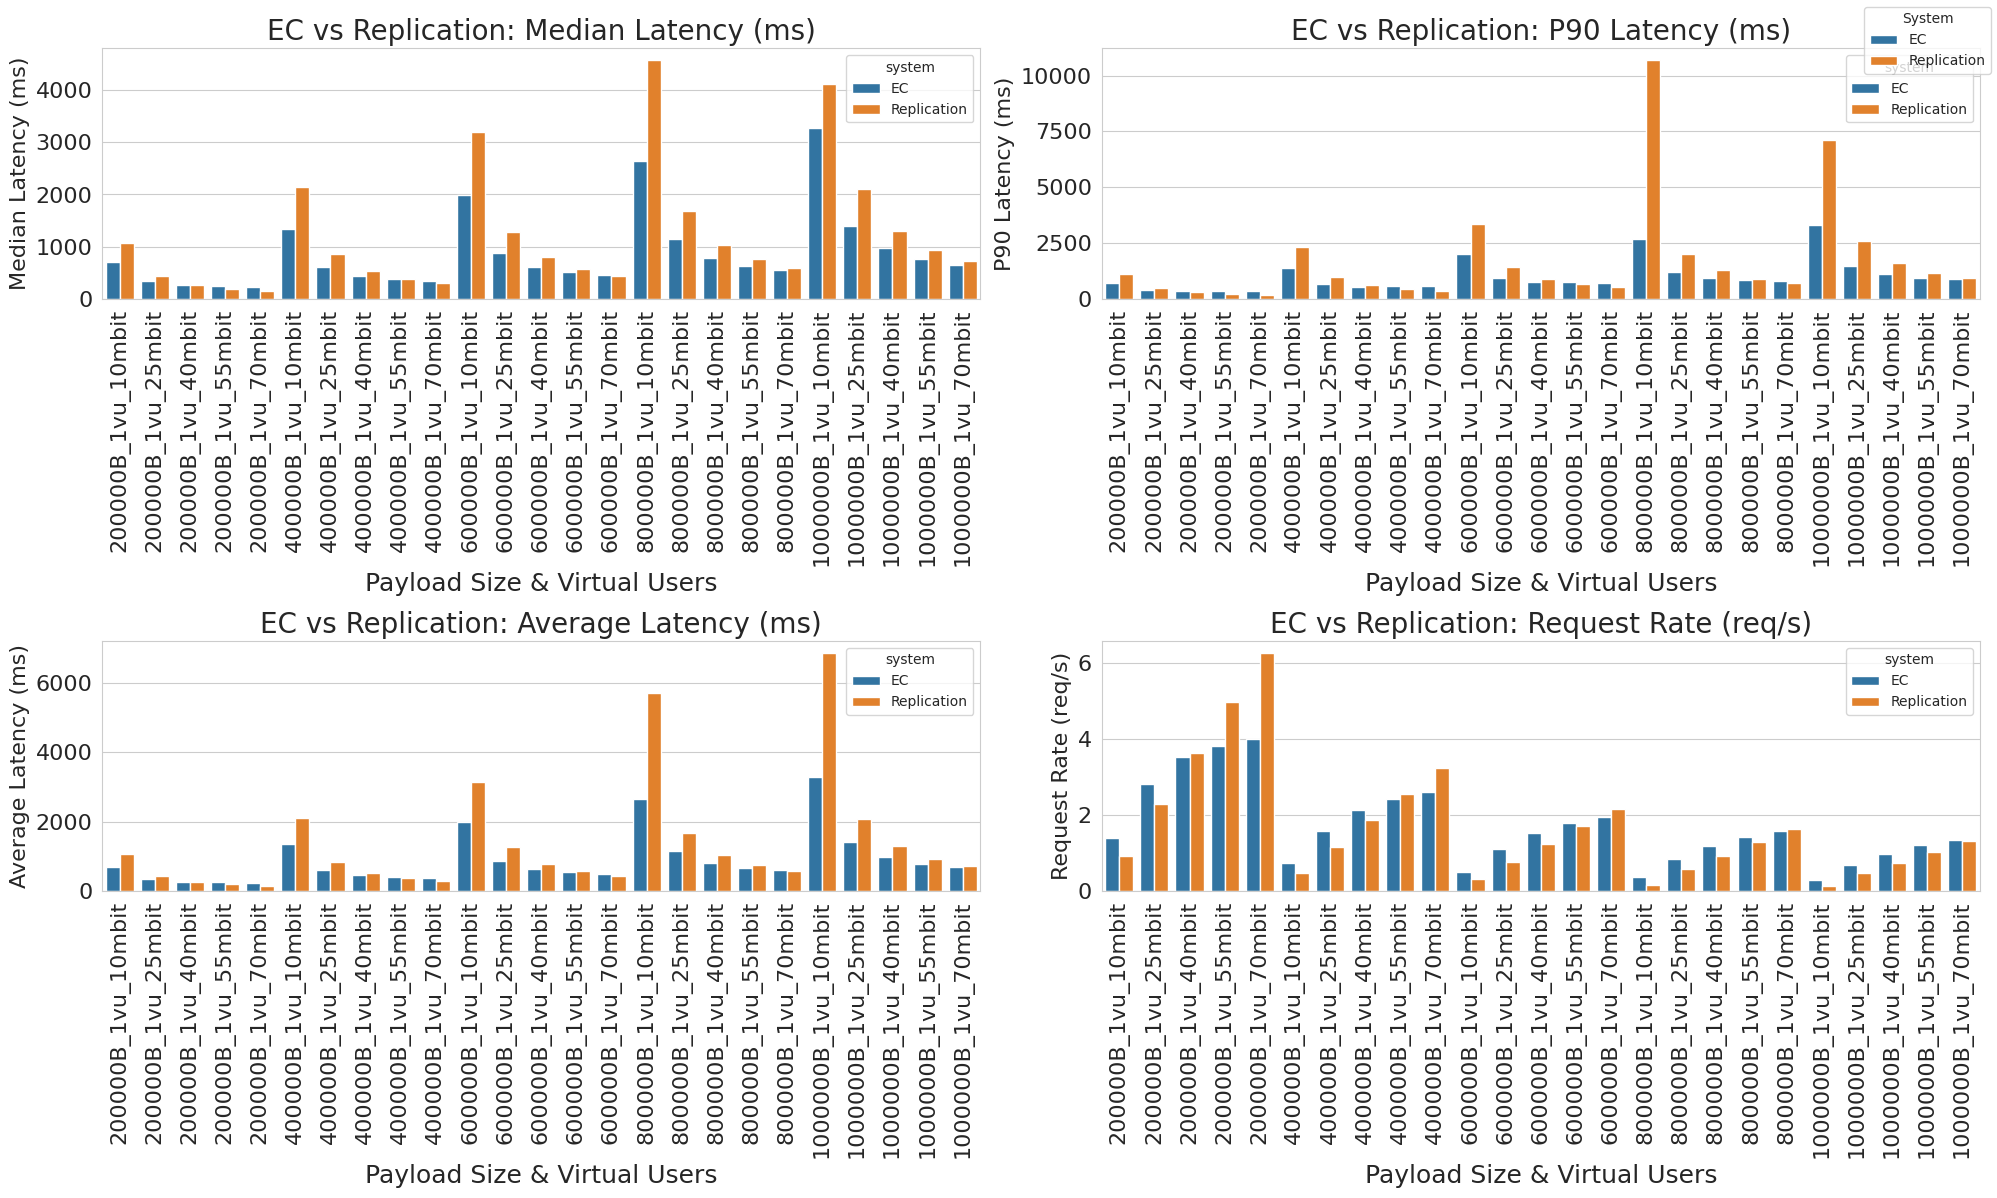
\includegraphics[width=0.8\textwidth]{resources/chapter-4/write_bigload_avgnet.png}

    \caption{Kinerja Write pada Internet Menengah dan Payload Besar}
    \label{fig:write-bigload-avgnet}
  \end{figure}

  Skenario ini menggunakan kombinasi \textit{payload} dan \textit{bandwidth} yang beragam sehingga memberikan diagram dengan grafik yang lebih kompleks. Gambar \ref{fig:write-bigload-avgnet} menunjukkan hasil \textit{benchmark} untuk skenario ini. Dari grafik tersebut, terlihat bahwa keunggulan \textit{erasure coding} semakin berkurang seiring dengan peningkatan \textit{bandwidth} dan penurunan ukuran \textit{payload}. Pada titik tertentu, sistem berbasis replikasi mulai mengungguli sistem berbasis \textit{erasure coding}. Titik impas terjadi ketika penghematan waktu dari transfer data yang lebih sedikit pada \textit{erasure coding} setara dengan penambahan waktu dari proses komputasi \textit{encoding}.

  \begin{figure}[ht]
    \centering
    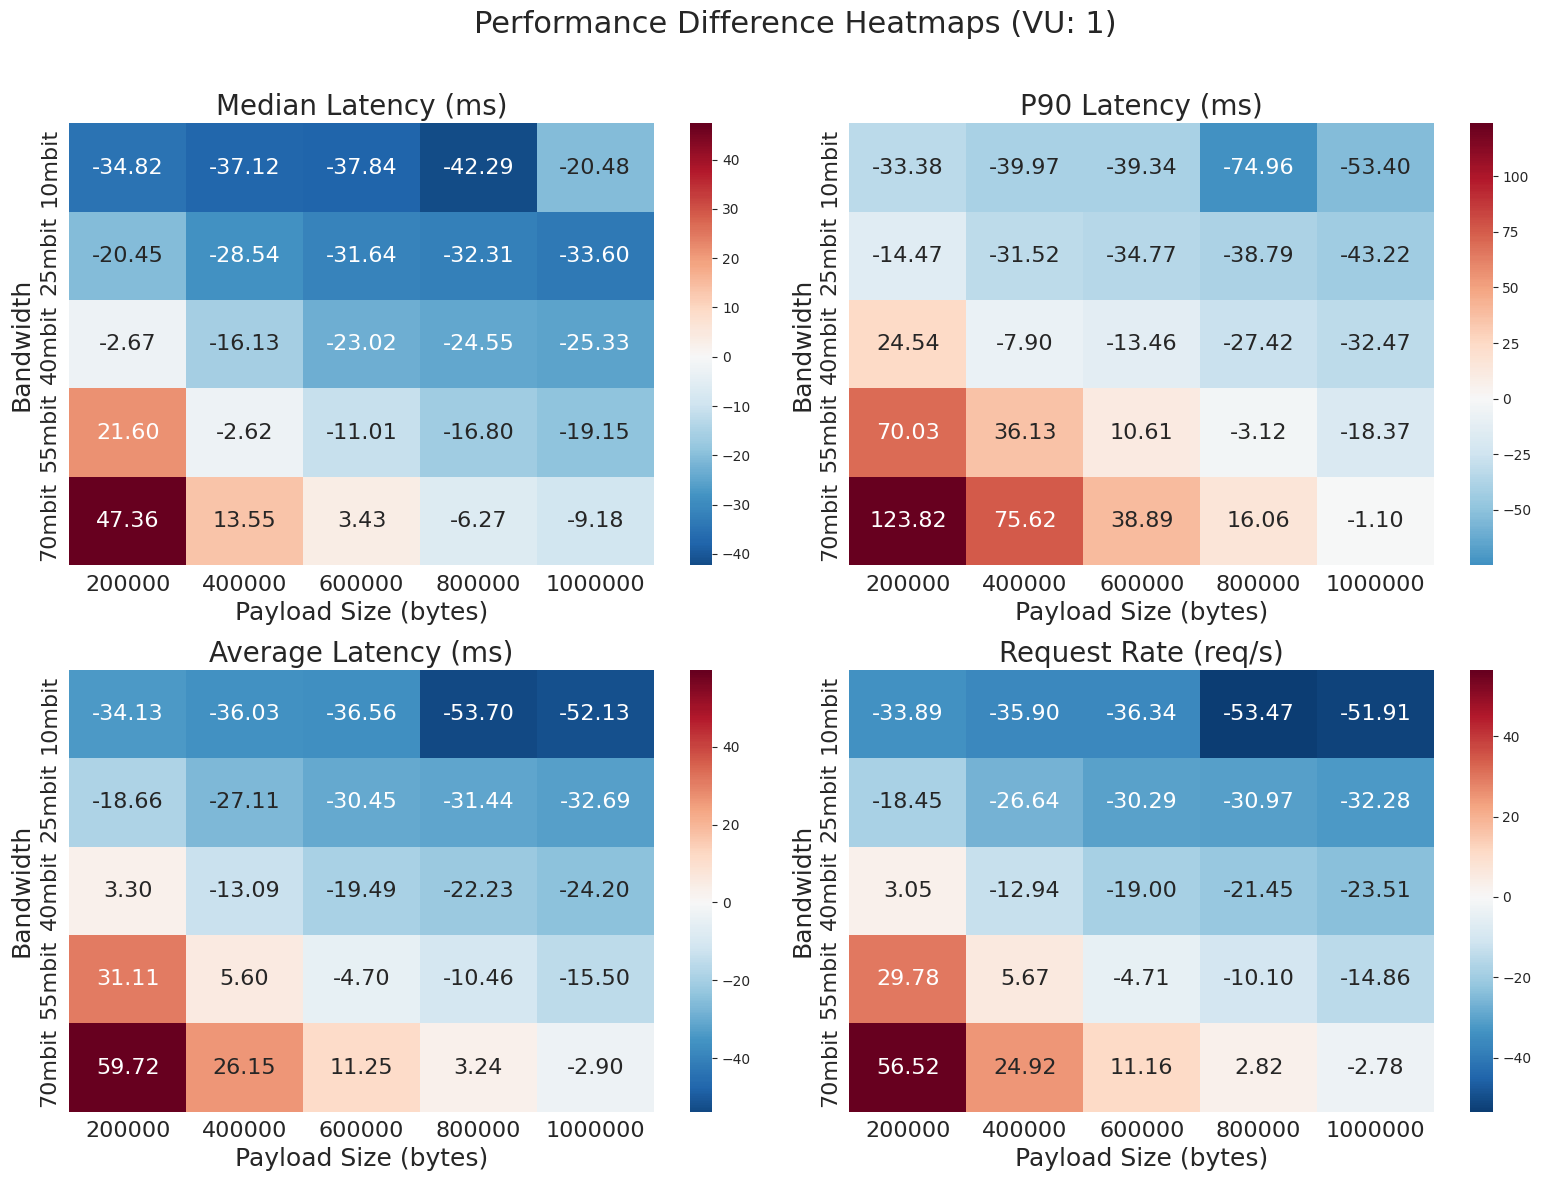
\includegraphics[width=0.8\textwidth]{resources/chapter-4/write_bigload_avgnet_heatmap.png}

    \caption{Heatmap Write pada Internet Menengah dan Payload Besar}
    \label{fig:write-bigload-avgnet-heatmap}
  \end{figure}

  Untuk memudahkan visualisasi, gambar \ref{fig:write-bigload-avgnet-heatmap} menunjukkan rasio kinerja dari hasil \textit{benchmark} terhadap \textit{payload} dan \textit{bandwidth} yang digunakan dalam persen. Warna biru dan nilai negatif menunjukkan keunggulan sistem berbasis \textit{erasure coding}, sedangkan warna merah dan nilai positif menunjukkan keunggulan sistem berbasis replikasi. Titik impas terlihat pada area transisi antara warna biru dan merah.  Kode yang digunakan untuk menghasilkan gambar ini dapat dilihat pada lampiran \ref{appendix:write-benchmark-code}. Transisi ini dapat dilihat pada gambar tersebut, namun tidak didapat titik yang tepat.

  Untuk menggambarkan perolehan titik impas, dapat dibuat diagram garis yang menunjukkan rata-rata \textit{response time} sistem berbasis \textit{erasure coding} dan replikasi terhadap \textit{bandwidth} dan ukuran \textit{payload}. Gambar \ref{fig:write-bigload-avgnet-line} menunjukkan diagram garis tersebut. Diagram ini memberikan gambaran visual yang jelas tentang bagaimana kinerja kedua sistem berubah seiring dengan variasi \textit{bandwidth} dan ukuran \textit{payload}.

  \begin{figure}[ht]
    \centering
    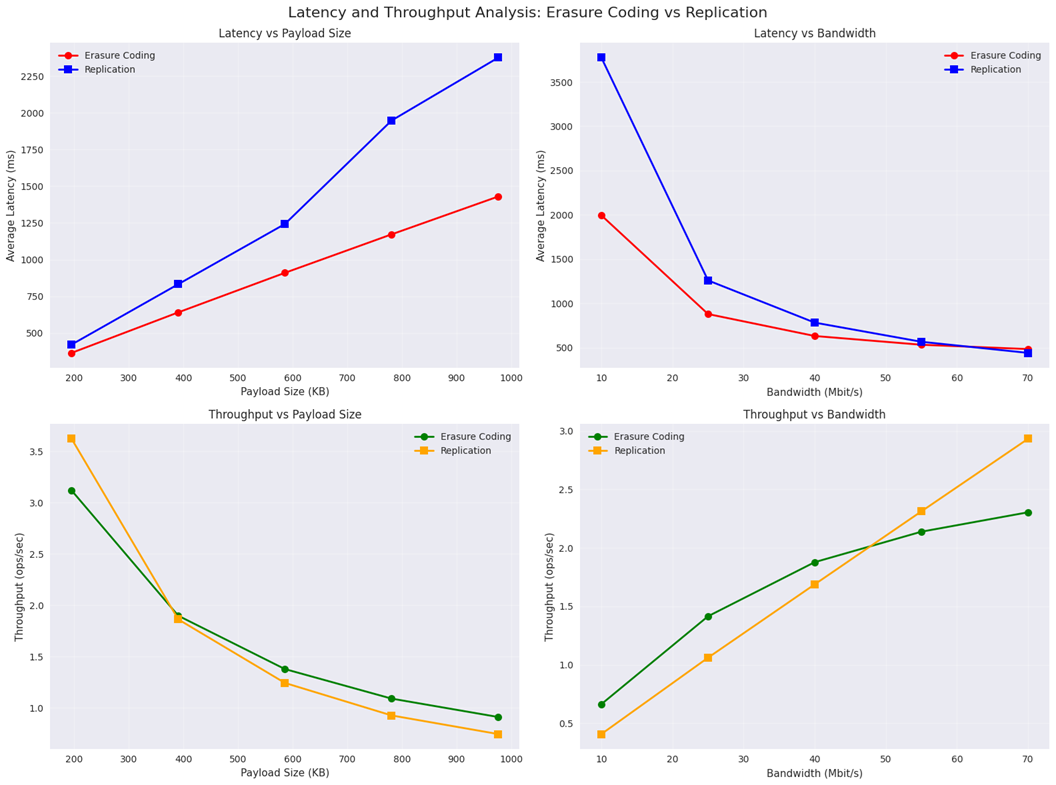
\includegraphics[width=0.8\textwidth]{resources/chapter-4/write_bigload_avgnet_line.png}

    \caption{Diagram Garis Write pada Internet Menengah dan Payload Besar}
    \label{fig:write-bigload-avgnet-line}
  \end{figure}

  
  Namun, untuk mendapatkan nilai yang tepat untuk titik impas antara sistem berbasis \textit{erasure coding} dan sistem berbasis replikasi, perlu dilakukan analisis lebih lanjut. Analisis untuk mendapatkan titik impas dilakukan secara menurunkan hasil \textit{benchmark} yang sudah dilakukan menjadi fungsi menggunakan pendekatan regresi. Fungsi ini kemudian digunakan untuk memperkirakan titik impas. Sebelum melakukan regresi, perlu dilihat \textit{scatter plot} dari hasil \textit{benchmark} sebagai gambaran visual relasi antara \textit{bandwidth}, ukuran \textit{payload}, dan \textit{response time}. Gambar \ref{fig:write-bigload-avgnet-scatter} menunjukkan \textit{scatter plot} tersebut.

  \begin{figure}[ht]
    \centering
    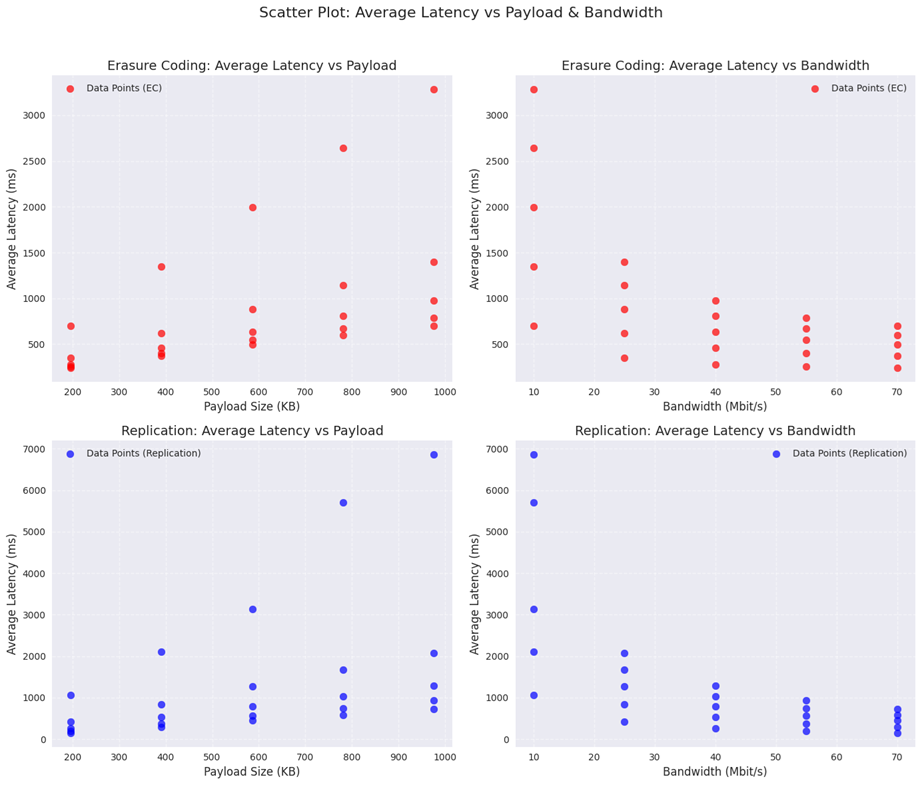
\includegraphics[width=0.8\textwidth]{resources/chapter-4/write_bigload_avgnet_scatterplot.png}

    \caption{Scatter Plot Write pada Internet Menengah dan Payload Besar}
    \label{fig:write-bigload-avgnet-scatter}
  \end{figure}

  Dari \textit{scatter plot} tersebut, terlihat bahwa hubungan dari \textit{bandwidth} dan ukuran \textit{payload} terhadap \textit{response time} tidak linear. Data yang dimiliki hanya sedikit, yaitu 25 data, sehingga regresi yang dilakukan harus mempertimbangkan risiko \textit{overfitting} yang tinggi. Selain itu, disebabkan lingkungan eksperimen dilakukan pada komputer pribadi, \textit{noise} dari eksperimen dapat mempengaruhi hasil. Dengan mempertimbangkan semua hal tersebut, regresi dilakukan dengan model \textit{ridge regression}. Model ini dipilih karena dapat menangani data yang memiliki banyak \textit{noise} serta mengurangi risiko \textit{overfitting} dengan menambahkan bias pada model regresi.

  Model \textit{ridge regression} gabungan dari \textit{bandwidth} dan \textit{payload} terhadap \textit{response time} menghasilkan model tiga dimensi seperti yang ditunjukkan pada gambar \ref{fig:write-bigload-avgnet-regression}.

  \begin{figure}[ht]
    \centering
    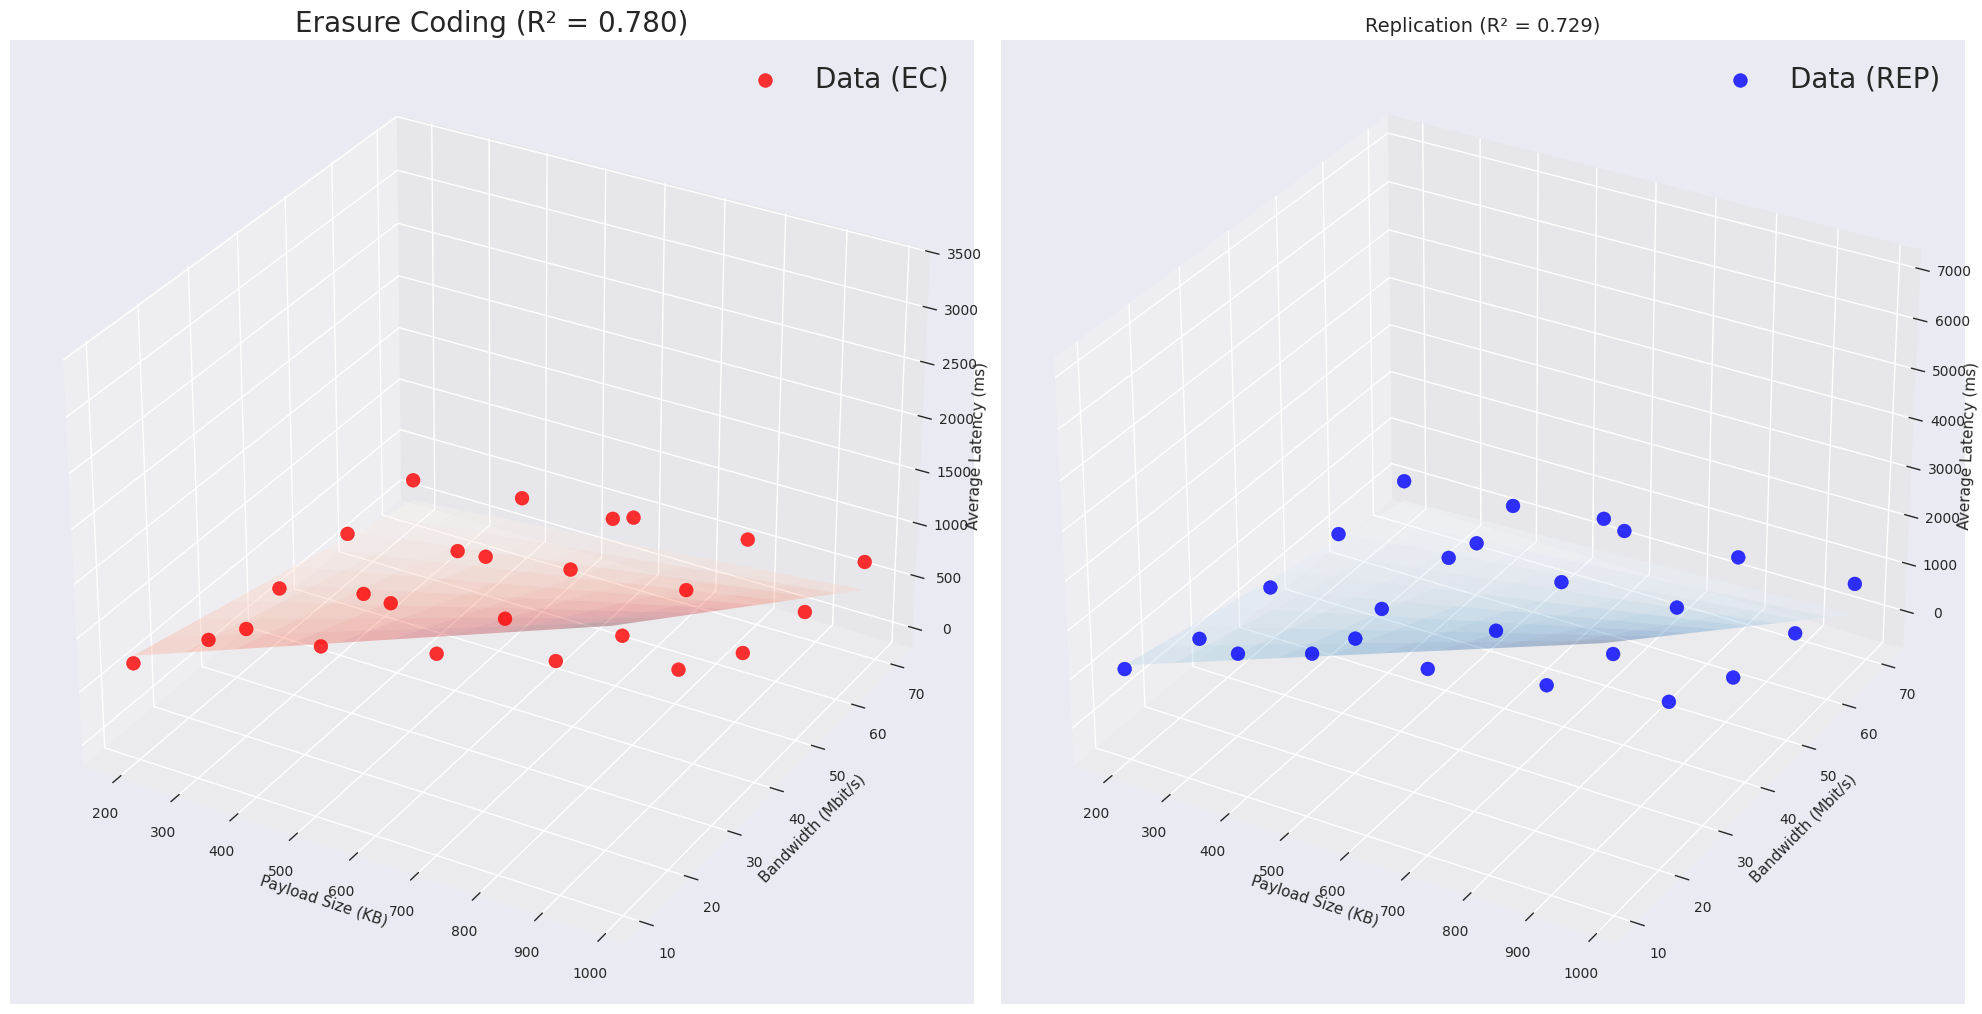
\includegraphics[width=0.8\textwidth]{resources/chapter-4/write_bigload_avgnet_regression.png}

    \caption{Model Regresi Operasi Write}
    \label{fig:write-bigload-avgnet-regression}
  \end{figure}

  Dari model regresi yang dilakukan, kurva pendekatan titik impas antara sistem berbasis \textit{erasure coding} dan sistem berbasis replikasi dapat dihasilkan dengan mencari perpotongan dari model regresi tersebut. Perpotongan didapat dengan menggunakan selisih dan selisih bernilai nol merupakan titik impas. Gambar \ref{fig:write-bigload-avgnet-boundary} menunjukkan analisis titik impas yang dilakukan dengan menggunakan model regresi. Dari perpotongan tersebut dapat dimodelkan menjadi persamaan kurva matematis yang dapat digunakan untuk memperkirakan titik impas pada \textit{bandwidth} dan ukuran \textit{payload} tertentu dengan nilai di atas kurva berarti sistem berbasis \textit{erasure coding} mengungguli sistem berbasis replikasi, dan nilai di bawah kurva berarti sebaliknya.


  \begin{figure}[ht]
    \centering
    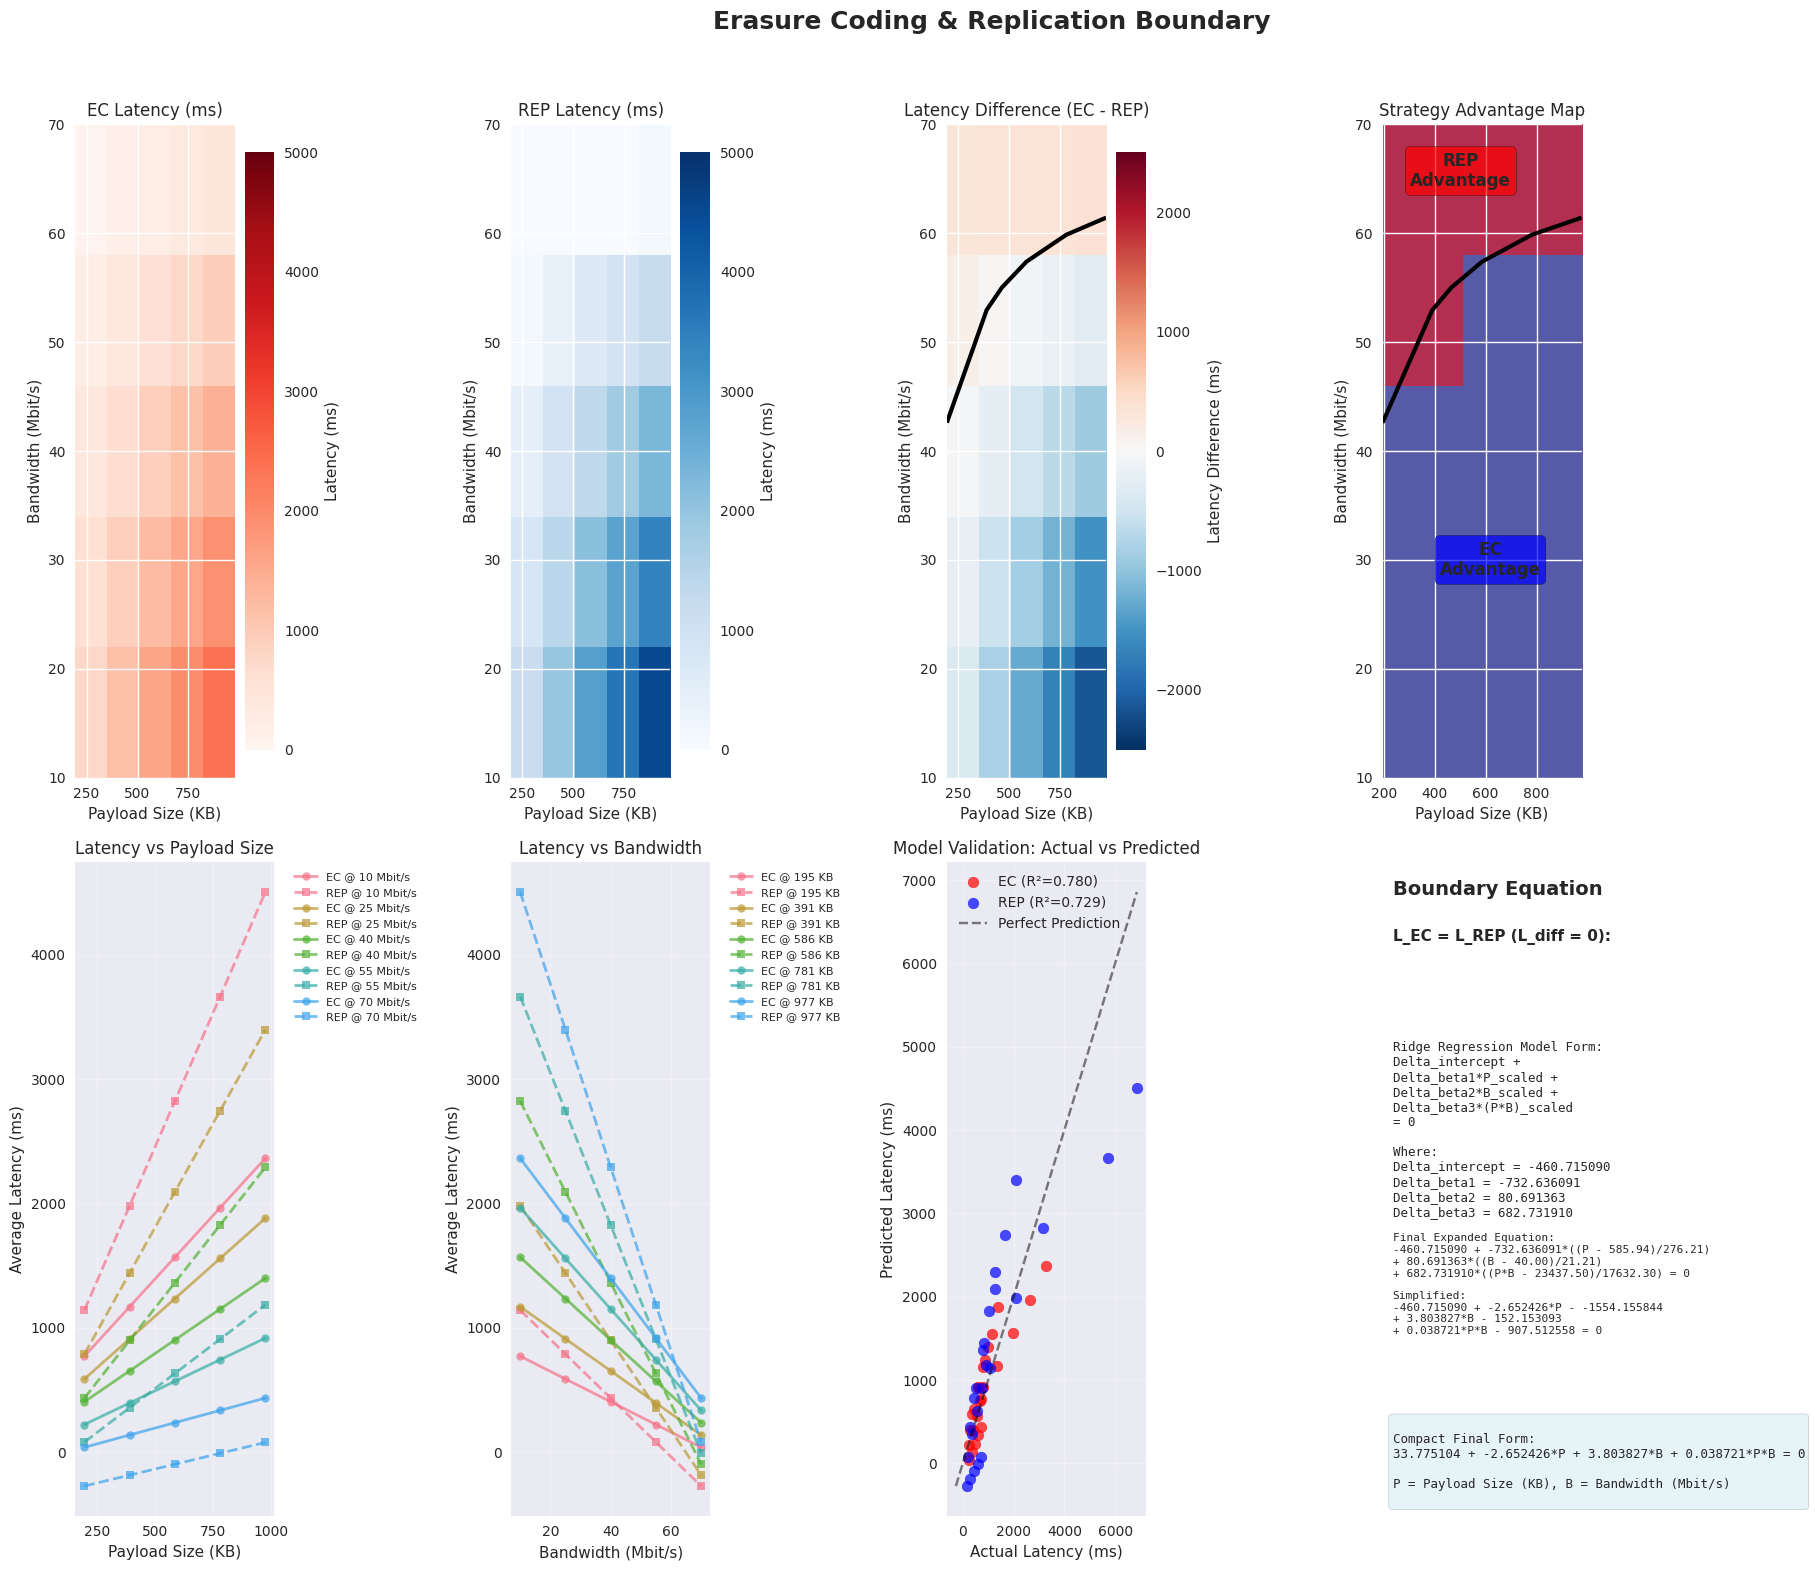
\includegraphics[width=\textwidth]{resources/chapter-4/write_bigload_avgnet_boundary.png}

    \caption{Analisis Titik Impas pada Operasi Write}
    \label{fig:write-bigload-avgnet-boundary}
  \end{figure}

  Kode yang digunakan untuk melakukan regresi ini dapat dilihat pada lampiran \ref{appendix:write-regression-code}. Perlu diketahui juga bahwa model regresi ini tidak mempertimbangkan faktor lain seperti kecepatan komputasi dari sistem yang digunakan, kecepatan akses memori, kecepatan akses disk, ataupun faktor lain yang dapat mempengaruhi \textit{response time}. Model ini hanya valid pada kondisi dan lingkungan eksperimen yang dilakukan.

\end{enumerate}

\subsubsection{Analisis Operasi Read}
\label{subsubsection:analisis-operasi-read}

Berbeda secara hipotesis dengan operasi \textit{write}, hipotesis kinerja operasi \textit{read} adalah bahwa replikasi akan secara konsisten menunjukkan kinerja yang lebih unggul dalam kondisi normal. Hal ini disebabkan oleh kompleksitas \textit{erasure coding} yang membutuhkan rekonstruksi data dari beberapa bagian, sedangkan replikasi dapat mengembalikan data secara langsung dari salinan pada \textit{node} tersebut.

Pada implementasi yang dijelaskan pada Bagian \ref{subsubsection:implementasi-memory-store}, dibuat sebuah \textit{in-memory store} untuk mengurangi latensi \textit{read} dengan mengurangi operasi rekonstruksi data. Jika menggunakan hal tersebut, \textit{erasure coding} akan memiliki kinerja yang setara dengan replikasi ketika data yang dibutuhkan sudah ada di \textit{in-memory store}. Untuk keperluan analisis ini, \textit{in-memory store} diabaikan dan semua \textit{request} yang diterima perlu direkonstruksi terlebih dahulu pada sistem \textit{erasure coding}.

Analisis ini bertujuan untuk mengukur seberapa buruk kinerja operasi \textit{read} pada sistem \textit{erasure coding} dibandingkan dengan replikasi. Sama seperti analisis operasi \textit{write}, analisis ini akan dibagi berdasarkan skenario yang sudah disebutkan pada Bagian \ref{subsubsection:setup-benchmark}. Setiap skenario akan dianalisis berdasarkan hasil \textit{benchmark} yang telah dilakukan.

\begin{enumerate}
  \item Skenario 1: Internet cepat dan \textit{payload} kecil
  
  Pada skenario pertama yang dirancang sebagai kondisi ekstrem yang menguntungkan replikasi, hasil \textit{benchmark} menunjukkan bahwa sistem replikasi memiliki \textit{response time} yang lebih rendah dibandingkan sistem berbasis \textit{erasure coding}. Skenario ini mengkonfirmasi hipotesis bahwa replikasi akan lebih cepat dalam kondisi internet cepat dan \textit{payload} kecil untuk operasi \textit{read}.
  
  Tidak banyak yang dapat disimpulkan dari hasil ini, karena skenario ini dirancang untuk menguntungkan replikasi dan dengan hipotesis menyebutkan bahwa replikasi akan selalu lebih cepat dalam kondisi apapun dibandingkan dengan \textit{erasure coding} untuk operasi \textit{read}. Skenario ini adalah salah satu dari kemungkinan kondisi untuk menjalankan sistem berbasis \textit{erasure coding} ataupun replikasi. Perbedaan kinerja ini dapat dilihat pada Gambar \ref{fig:read-smload-fastnet}.

  \begin{figure}[ht]
    \centering
    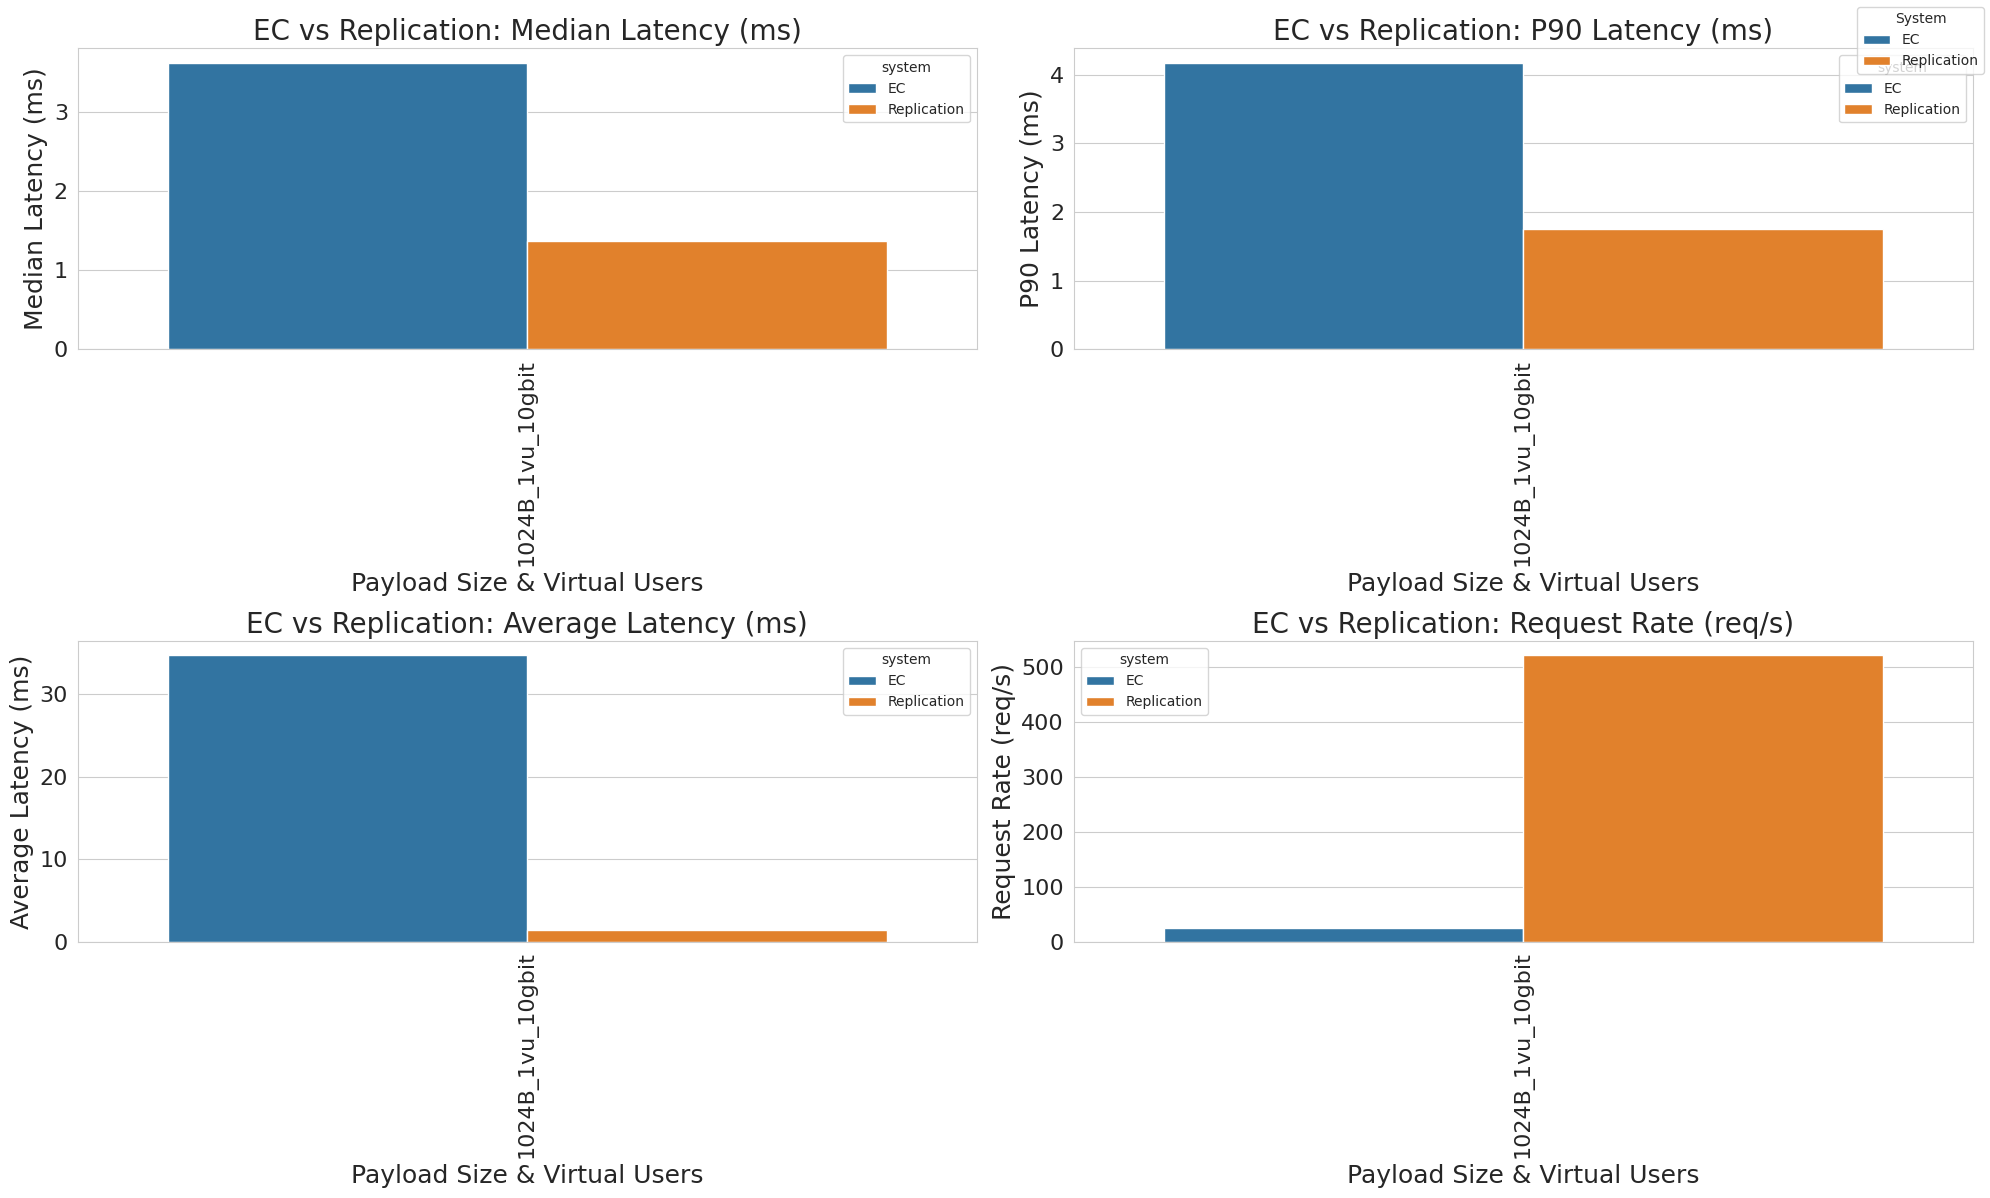
\includegraphics[width=0.8\textwidth]{resources/chapter-4/read_smload_fastnet.png}

    \caption{Kinerja Operasi Read pada Internet Cepat dan Payload Kecil}
      \label{fig:read-smload-fastnet}
  \end{figure}

  Proses \textit{erasure coding} memerlukan rekonstruksi data sehingga kinerjanya selalu lebih lambat dibandingkan replikasi. Grafik tersebut memperlihatkan kinerja \textit{erasure coding} dan replikasi memiliki perbedaan yang signifikan.

  \item Skenario 2: Internet lambat dan \textit{payload} besar
  
  Skenario kedua berlawanan dengan skenario pertama pada operasi \textit{write}. Namun, kondisi ini tidak berlaku untuk operasi \textit{read}. Gambar \ref{fig:read-bigload-slownet} menunjukkan hasil \textit{benchmark} untuk skenario ini.

  \begin{figure}[ht]
    \centering
    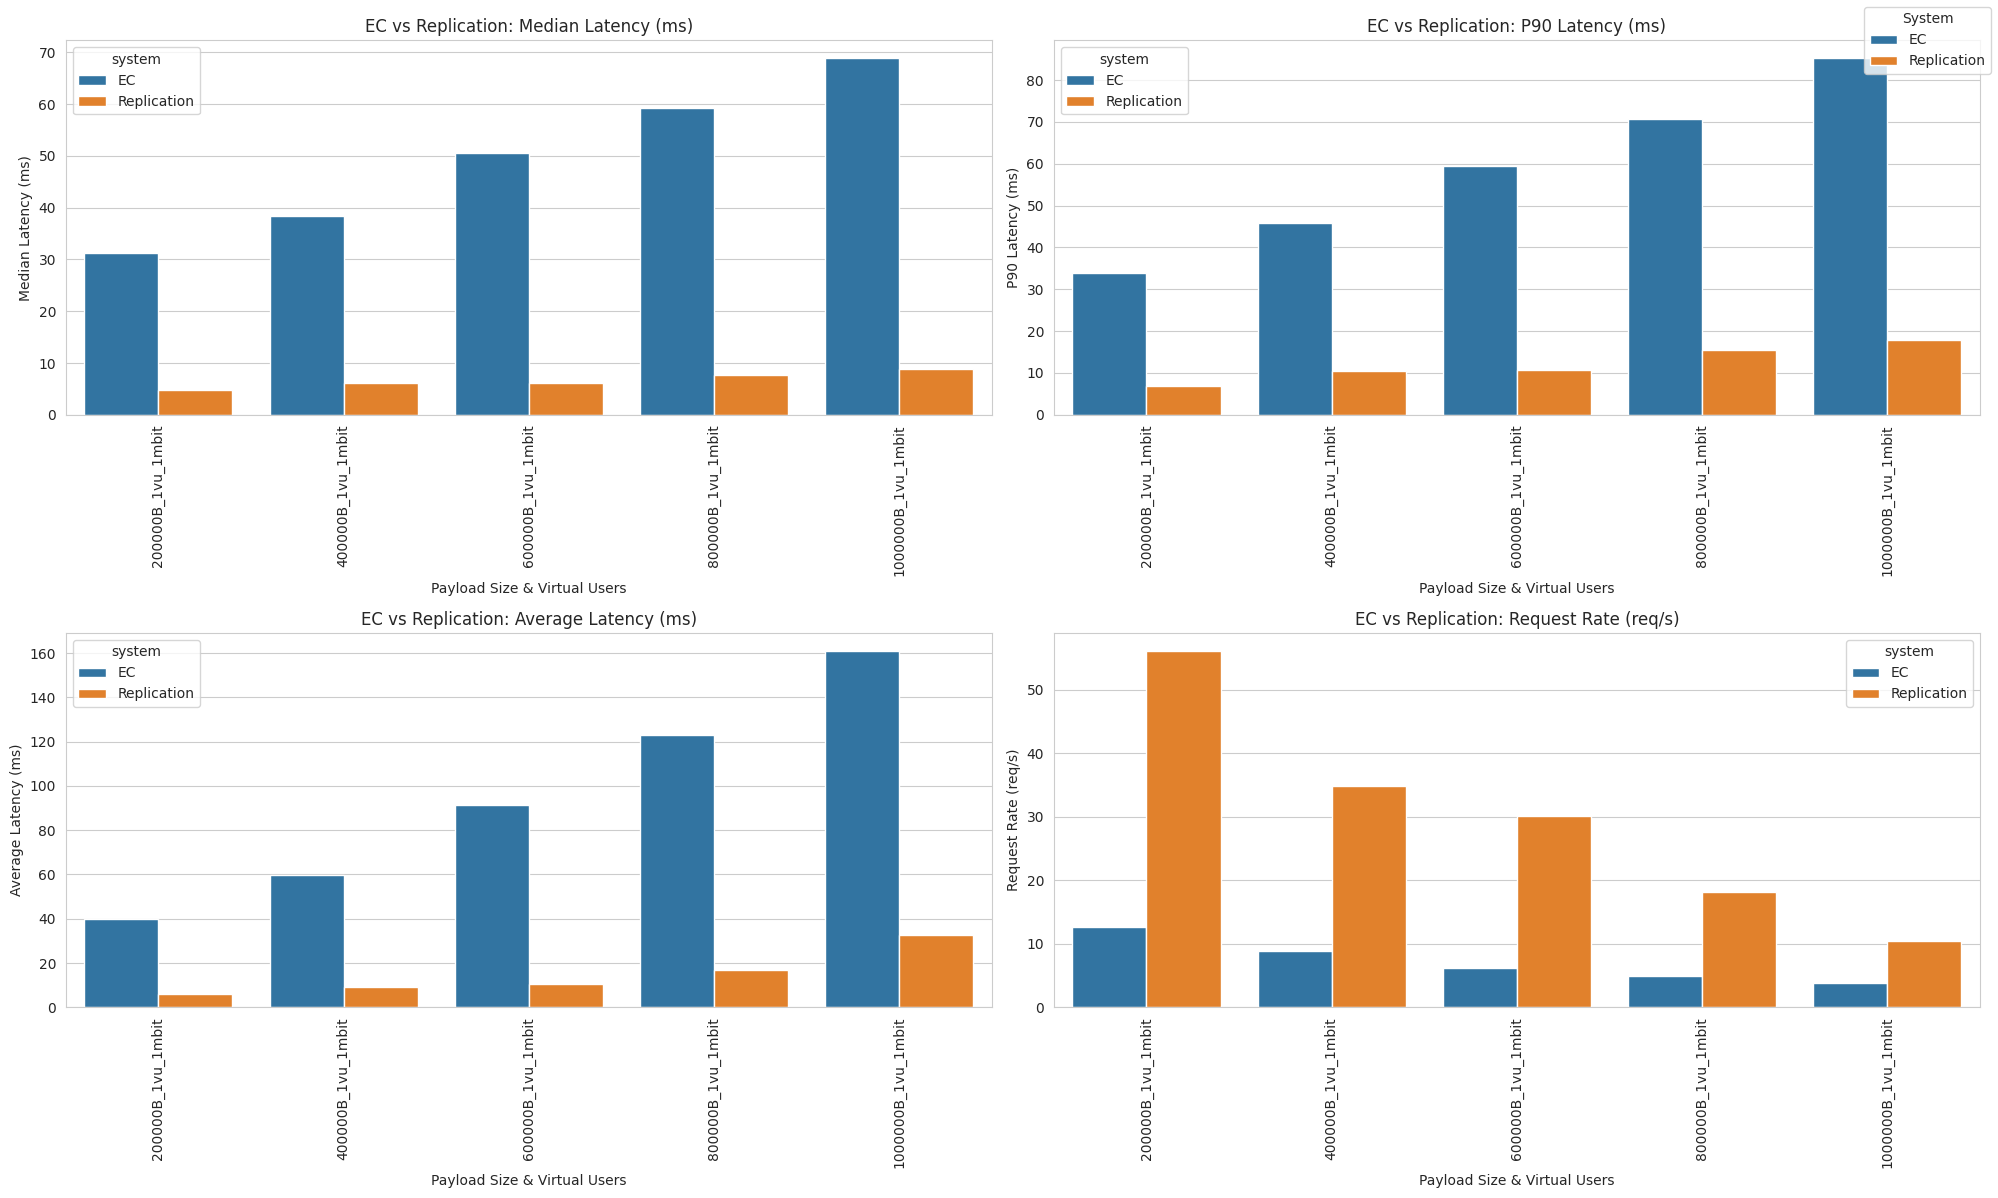
\includegraphics[width=0.8\textwidth]{resources/chapter-4/read_bigload_slownet.png}

    \caption{Kinerja Operasi Read pada Internet Lambat dan Payload Besar}
      \label{fig:read-bigload-slownet}
  \end{figure}

  Hasil dari skenario ini mengkonfirmasi bahwa \textit{erasure coding} tidak dapat mengungguli replikasi dalam kondisi apapun untuk operasi \textit{read}. Proses rekonstruksi data pada sistem \textit{erasure coding} akan tetap membutuhkan waktu yang lebih lama dibandingkan dengan replikasi, meskipun dalam kondisi internet lambat dan \textit{payload} besar. Selain itu, hasil ini menunjukkan juga bahwa keuntungan yang dimiliki \textit{erasure coding} dalam operasi \textit{write} perlu diiringi dengan penurunan kinerja pada operasi \textit{read}.

  \item Skenario 3: Internet menengah dan \textit{payload} besar
  
  Dari konfirmasi yang didapatkan dari kedua skenario sebelumnya bahwa \textit{erasure coding} tidak dapat mengungguli replilkasi untuk operasi \textit{read} dalam kondisi apapun, skenario ketiga melakukan eksplorasi tambahan terkait signifikansi perbedaan kinerja antar \textit{erasure coding} dan replikasi. Gambar \ref{fig:read-bigload-avgnet} menunjukkan hasil \textit{benchmark} untuk skenario ini.

  \begin{figure}[ht]
    \centering
    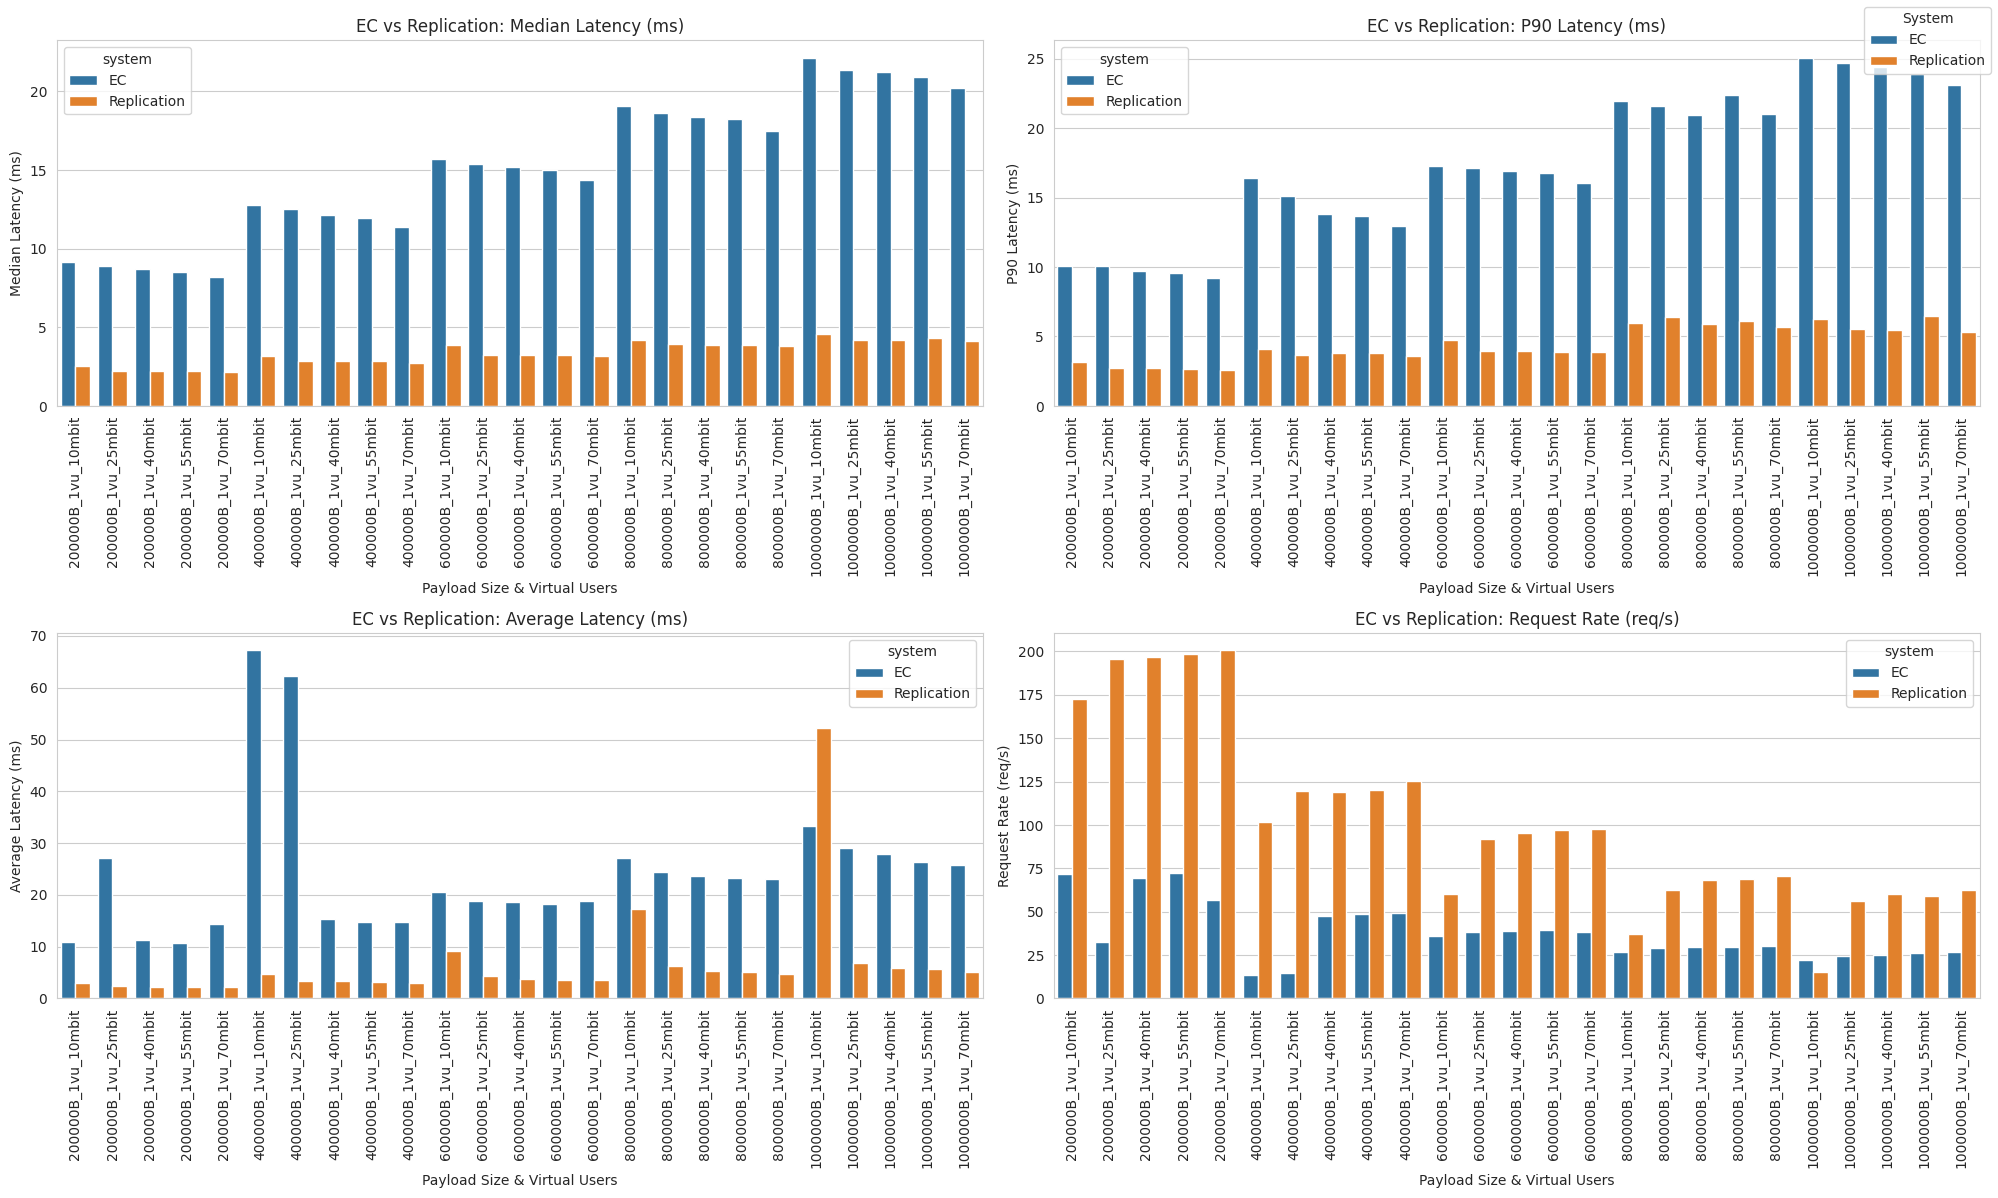
\includegraphics[width=0.8\textwidth]{resources/chapter-4/read_bigload_avgnet.png}

    \caption{Kinerja Operasi Read pada Internet Menengah dan Payload Besar}
      \label{fig:read-bigload-avgnet}
  \end{figure}

  Mengabaikan data \textit{noise} hasil \textit{benchmark}. Grafik tersebut menunjukkan perbedaan kinerja antara sistem berbasis \textit{erasure coding} dan replikasi secara umum menurun dengan \textit{payload} yang lebih kecil. Hal ini disebabkan oleh proses rekonstruksi data berjalan lebih cepat ketika \textit{payload} yang direkonstruksi lebih kecil dengan berkurangnya operasi yang perlu dilakukan dan juga pengiriman data antar-\textit{node}.

  Visualisasi \textit{heatmap} pada Gambar \ref{fig:read-bigload-avgnet-heatmap} menunjukkan perbedaan kinerja replikasi unggul pada operasi \textit{read}. Keunggulan ini semakin bertambah ketika \textit{payload} yang direkonstruksi semakin besar. Perubahan \textit{bandwidth} juga mempengaruhi kinerja \textit{erasure coding} dan replikasi. Penambahan \textit{bandwidth} menambah \textit{response time} dari kedua sistem, namun \textit{erasure coding} terlihat lebih terpengaruh dibandingkan replikasi. Hal ini disebabkan oleh proses rekonstruksi data yang membutuhkan pengumpulan \textit{fragment} dari beberapa \textit{node} terpisah terlebih dahulu melalui jaringan sebelum melakukan rekonstruksi, sedangkan replikasi hanya bertambah waktu yang diperlukan untuk mengirimkan data dari \textit{node} ke \textit{client}. Kode untuk visualisasi \textit{heatmap} dapat dilihat pada repository Github hasil implementasi.

  \begin{figure}[ht]
    \centering
    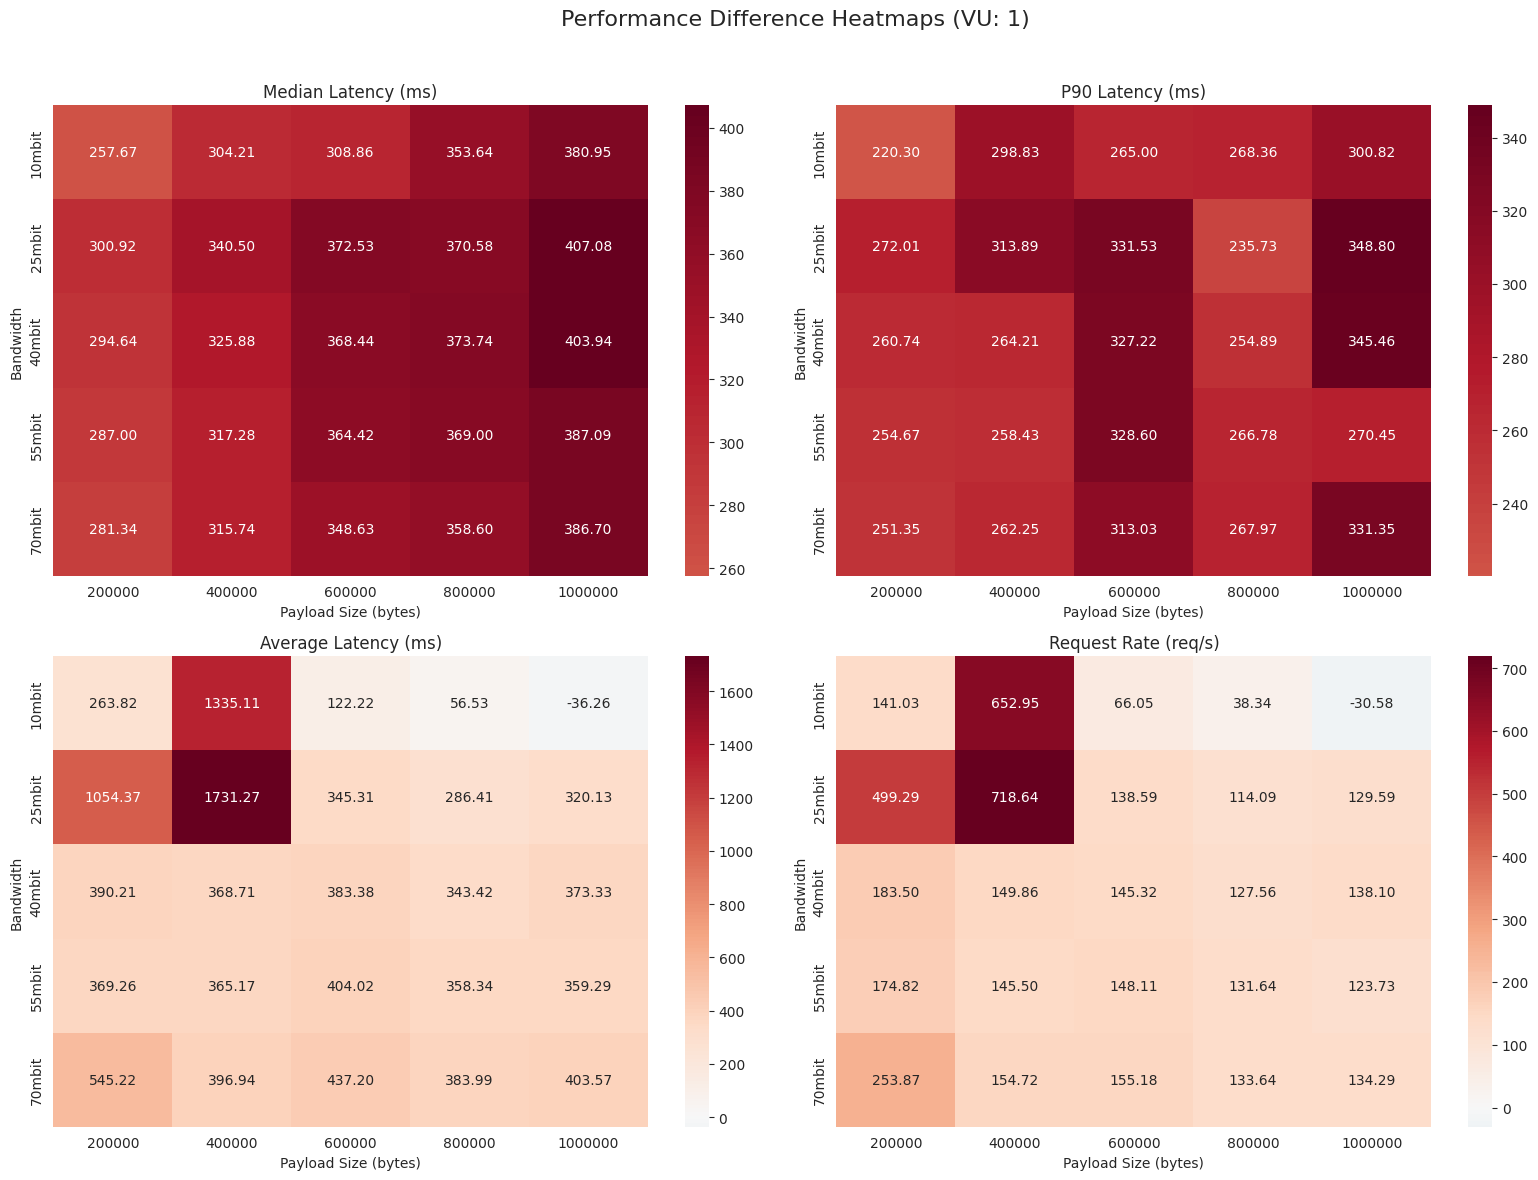
\includegraphics[width=0.8\textwidth]{resources/chapter-4/read_bigload_avgnet_heatmap.png}

    \caption{Heatmap Read pada Internet Menengah dan Payload Besar}
      \label{fig:read-bigload-avgnet-heatmap}
  \end{figure}

  Jike dibentuk diagram garis untuk memvisualisasikan pendekatan kinerja operasi \textit{read} pada sistem berbasis \textit{erasure coding} dan replikasi. Terlihat bahwa diagram garis yang dibentuk tidak menunjukkan \textit{trajectory} bahwa garis akan bersinggungan dengan garis \textit{erasure coding} pada titik tertentu. Perbandingan kinerja replikasi dan \textit{erasure coding} pada operasi \textit{read} memiliki kurva yang berbeda dan tidak akan bersinggungan. Diagram garis ini dapat dilihat pada Gambar \ref{fig:read-bigload-avgnet-line}.

  \begin{figure}[ht]
    \centering
    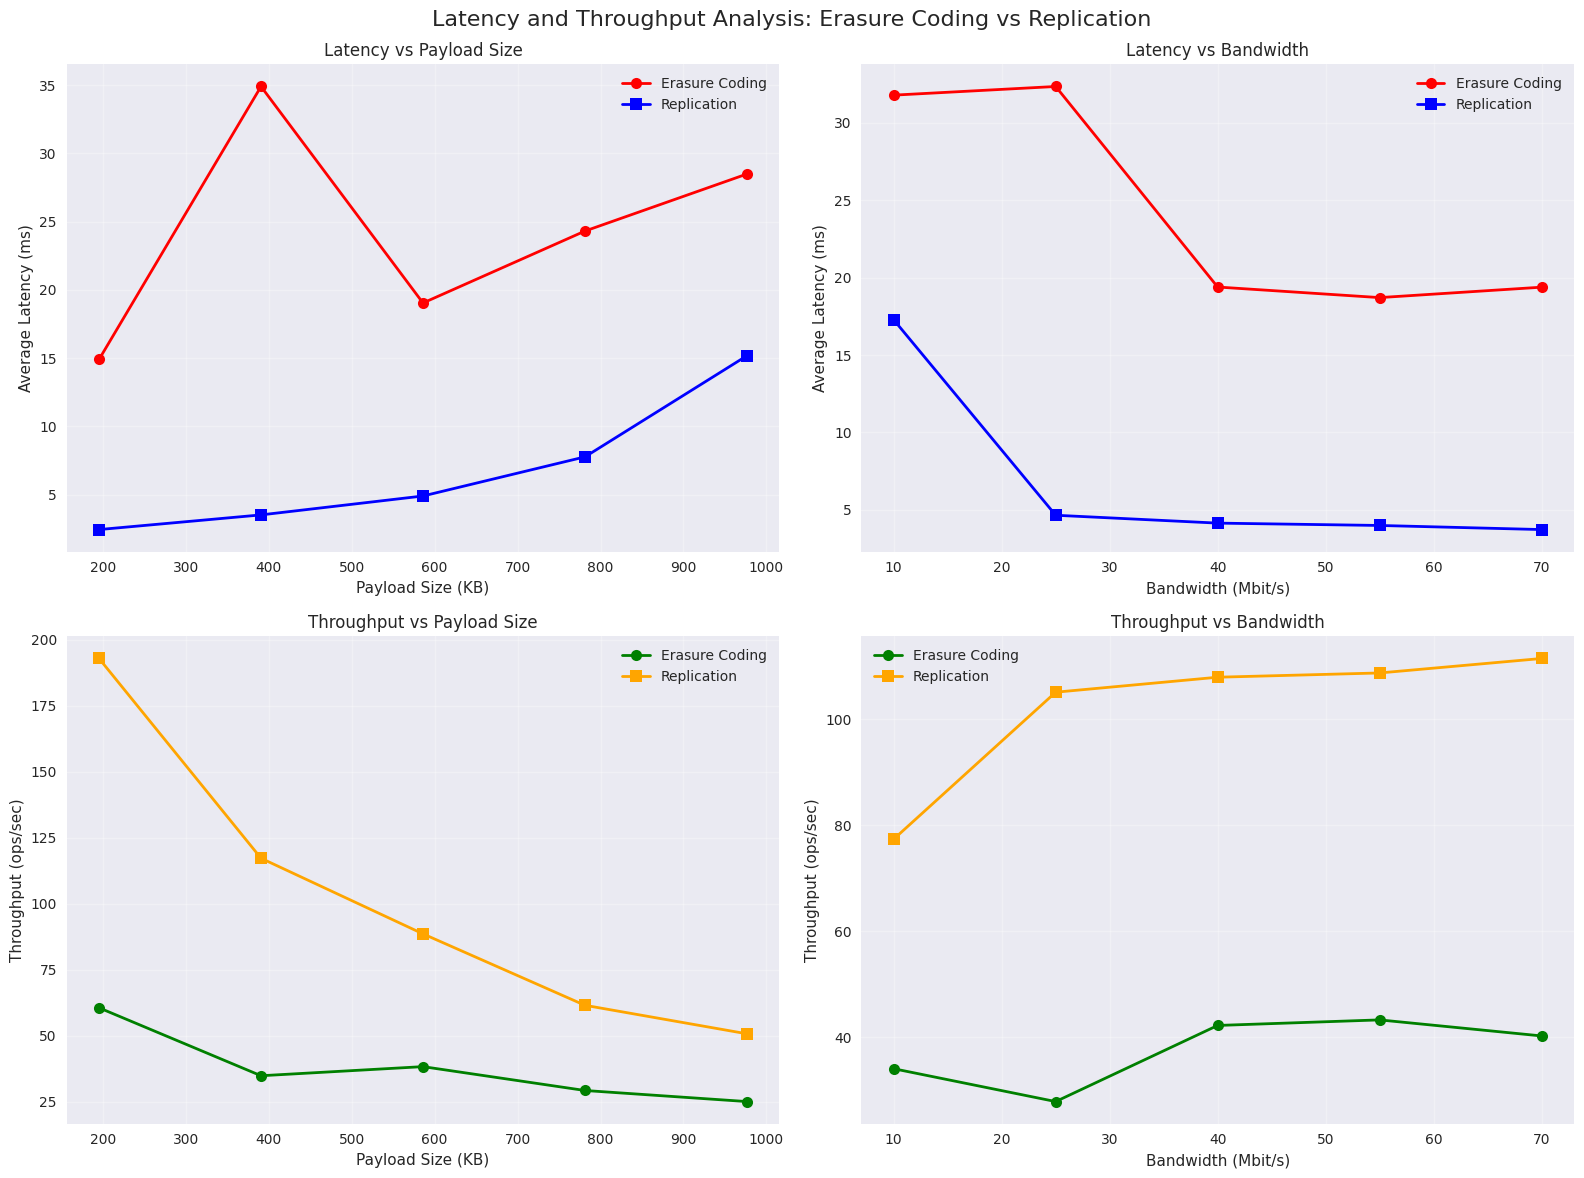
\includegraphics[width=0.8\textwidth]{resources/chapter-4/read_bigload_avgnet_line.png}

    \caption{Diagram Garis Read pada Internet Menengah dan Payload Besar}
    \label{fig:read-bigload-avgnet-line}
  \end{figure}

  Pembuktian matematis sederhana dapat dilakukan untuk menyatakan bahwa kinerja \textit{erasure coding} tidak akan pernah mengungguli replikasi pada operasi \textit{read}. Erasure coding akan membutuhkan waktu untuk memberikan data pada \textit{client}, rekonstruksi, dan meminta \textit{shard} pada \textit{node} lainnya, sedangkan replikasi hanya membutuhkan waktu untuk memberikan data pada \textit{client}. Persamaan \ref{eq:ec-read-latency} dan Persamaan \ref{eq:rep-read-latency} menunjukkan perhitungan latensi operasi \textit{read} pada sistem berbasis \textit{erasure coding}.

  \begin{align}
  L_{EC} &= T_{data} + T_{rekonstruksi} + T_{shard}
  \label{eq:ec-read-latency}
  \end{align}

  Sementara itu, Persamaan \ref{eq:rep-read-latency} menunjukkan perhitungan latensi operasi \textit{read} pada sistem berbasis replikasi.

  \begin{align}
  L_{REP} &= T_{data}
  \label{eq:rep-read-latency}
  \end{align}

  Dari persamaan tersebut, waktu antara \textit{erasure coding} dan replikasi dapat dituliskan sebagai Persamaan \ref{eq:read-latency-diff}.

  \begin{align}
  \Delta L &= L_{EC} - L_{REP} \\
  &= (T_{data} + T_{rekonstruksi} + T_{shard}) - T_{data} \\
  &= T_{rekonstruksi} + T_{shard}
  \label{eq:read-latency-diff}
  \end{align}

  Dengan demikian, perbedaan waktu antara \textit{erasure coding} dan replikasi akan menjadi semakin besar relatif terhadap ukuran data ketika data direkonstruksi, ukuran data ketika pengiriman data, dan juga \textit{bandwidth} yang tersedia ketika pengiriman data.
  
  Penambahan \textit{in-memory store} akan menghilangkan penambahan waktu ini. Namun, tidak semua \textit{request} dapat dilayani menggunakan \textit{in-memory store} karena keterbatasan memory yang tersedia. Oleh karena itu, peningkatan kinerja \textit{in-memory store} relatif terhadap rasio \textit{hit} dan \textit{miss} dari \textit{key} yang diminta. Jika \textit{hit} adalah seratus persen, maka \textit{erasure coding} akan memiliki kinerja yang setara dengan replikasi. Penambahan \textit{in-memory store} memodifikasi Persamaan \ref{eq:ec-read-latency} menjadi Persamaan \ref{eq:ec-read-latency-inmemory}.

  \begin{align}
    L_{EC} &= T_{data} + (T_{rekonstruksi} + T_{shard}) \times (1 - \text{hit rate})
    \label{eq:ec-read-latency-inmemory}
  \end{align}

  Dari persamaan tersebut, penambahan waktu yang dibutuhkan untuk operasi \textit{read} pada sistem berbasis \textit{erasure coding} dapat dihitung dengan mengurangi waktu yang dibutuhkan untuk operasi \textit{read} pada sistem replikasi. Persamaan ini dapat dituliskan sebagai Persamaan \ref{eq:ec-read-latency-diff-inmemory}.

  \begin{align}
    \Delta L &= L_{EC} - L_{REP} \\
    &= \left[T_{data} + (T_{rekonstruksi} + T_{shard}) \times (1 - \text{hit rate})\right] - T_{data} \\
    &= (T_{rekonstruksi} + T_{shard}) \times (1 - \text{hit rate})
    \label{eq:ec-read-latency-diff-inmemory}
  \end{align}

  Penambahan \textit{in-memory store} akan mengurangi waktu operasi \textit{read} pada sistem berbasis \textit{erasure coding} dengan kemungkinan untuk mengimbangi kinerja replikasi. Namun, hal ini tergantung pada rasio \textit{hit} yang dapat dicapai oleh \textit{in-memory store}.
  
  % Jika analisis regresi yang mirip dengan analisis pada Bagian \ref{subsubsection:analisis-operasi-write} dilakukan, hasil menunjukkan bahwa untuk semua skenario, \textit{erasure coding} memiliki kinerja yang lebih lambat dibandingkan replikasi. Grafik akhir dari analisis ini dapat dilihat pada Gambar \ref{fig:read-bigload-avgnet-regression}. Perlu diamati juga bahwa nilai \textit{R-squared} yang didapatkan dari analisis regresi ini adalah ada di bawah 0.5, yang menunjukkan bahwa model regresi ini tidak dapat menjelaskan variasi data dengan baik. Hal ini sebagian besar disebabkan oleh adanya \textit{noise} yang tinggi pada hasil \textit{benchmark}.

  % \begin{figure}[ht]
  %   \centering
  %   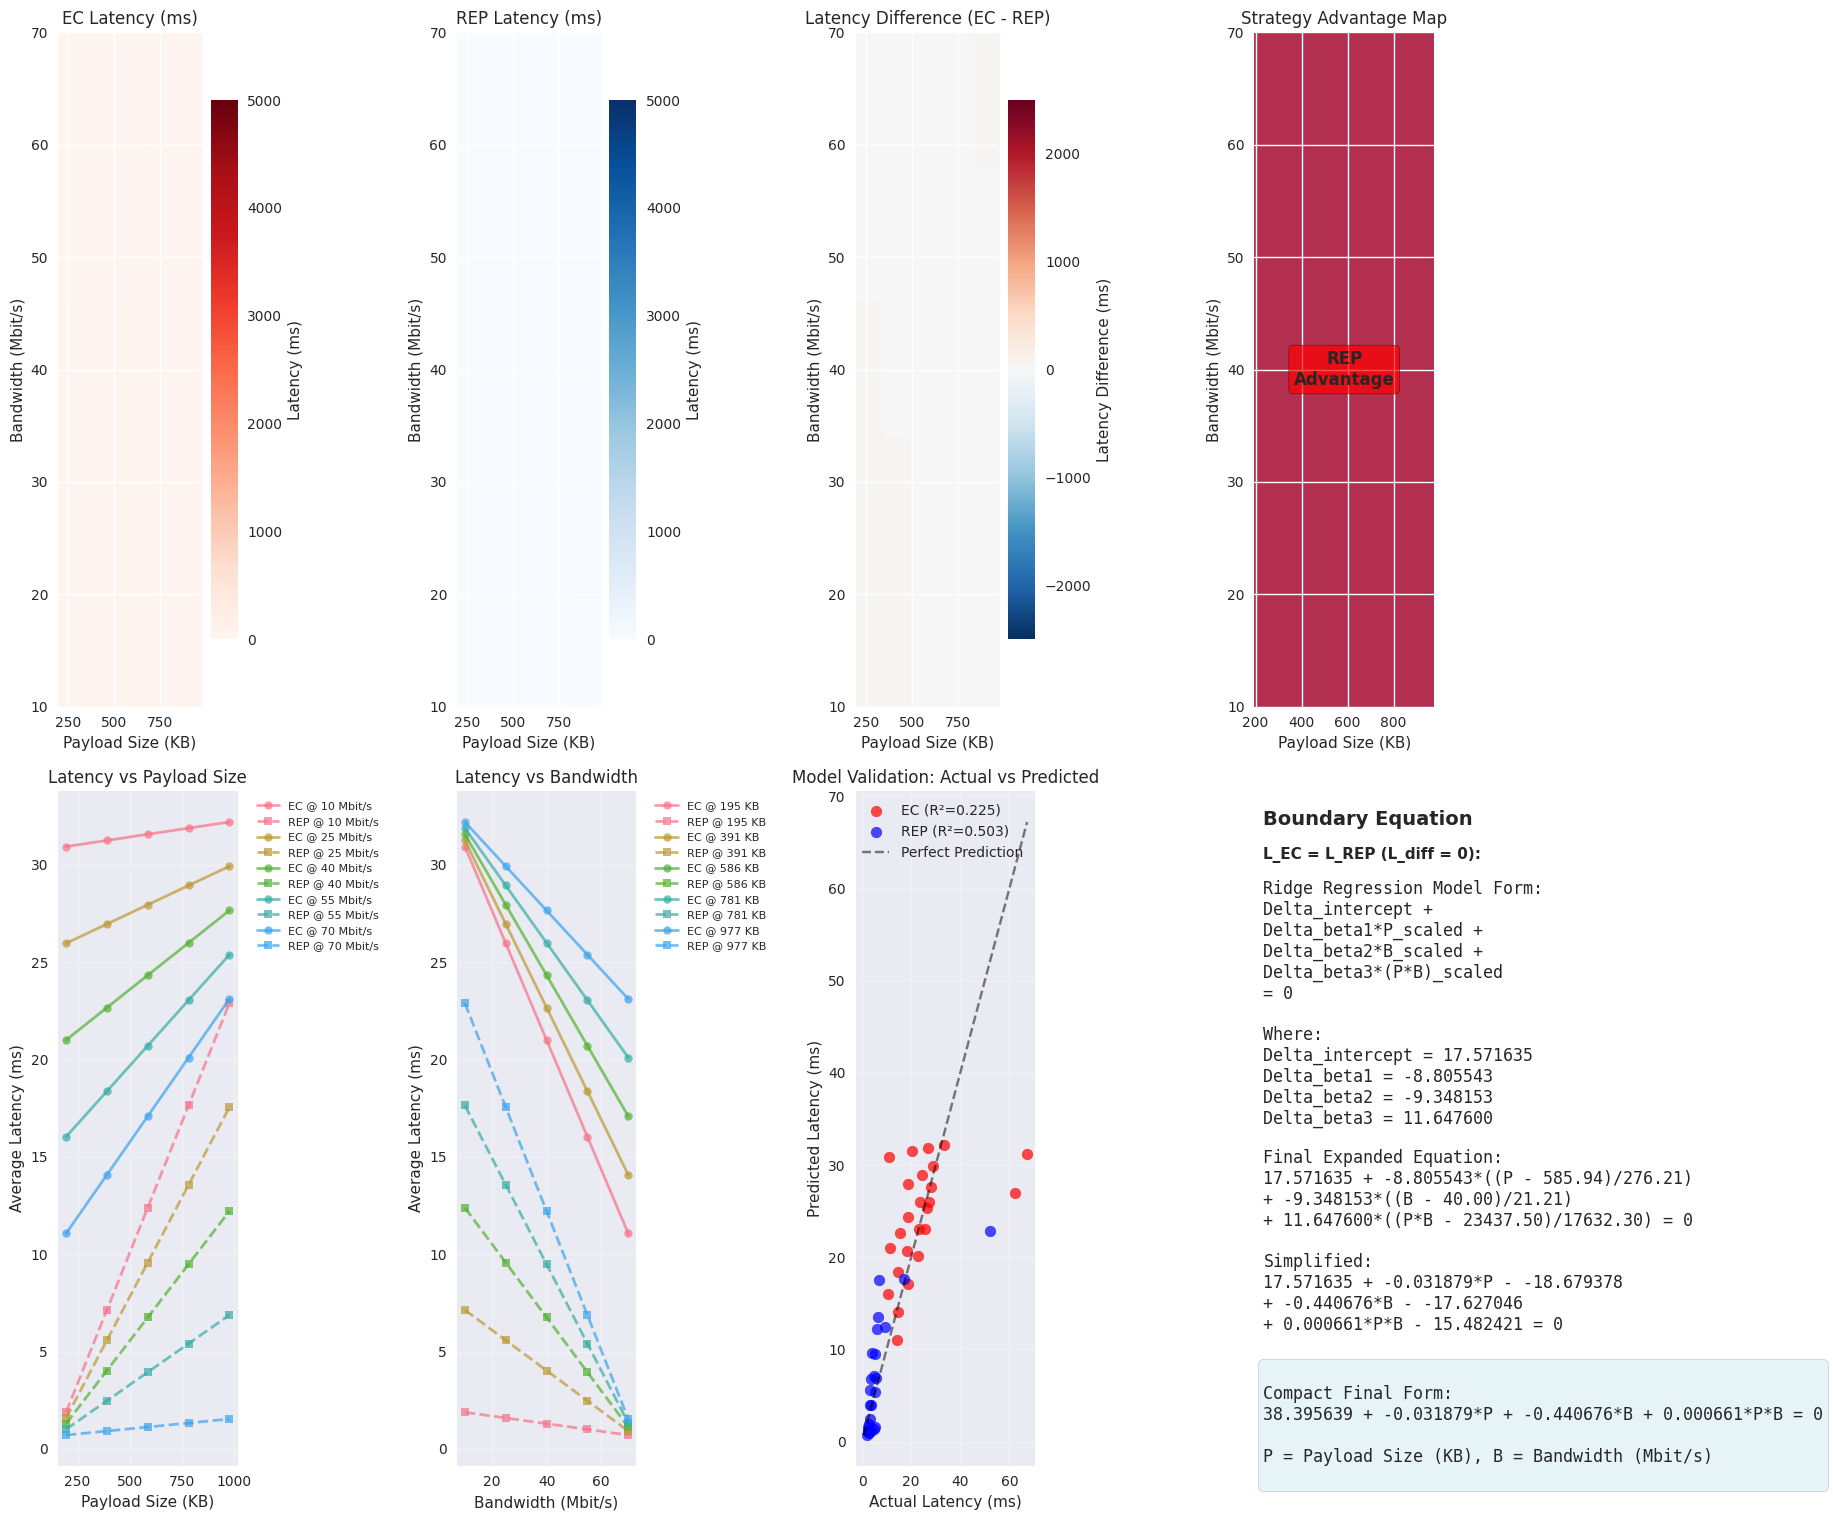
\includegraphics[width=0.8\textwidth]{resources/chapter-4/read_bigload_avgnet_regression.png}

  %   \caption{Analisis Regresi Read pada Internet Menengah dan Payload Besar}
  %   \label{fig:read-bigload-avgnet-regression}
  % \end{figure}
\end{enumerate}
\subsubsection{Analisis Keseluruhan}
\label{subsubsection:analisis-keseluruhan}

Setelah melakukan analisis terhadap dua operasi \textit{write} dan \textit{read}, bagian analisis ini menyatukan temuan dari evaluasi kinerja operasi tersebut. Tujuannya menyajikan gambaran keseluruhan mengenai \textit{trade-off} fundamental antara \textit{erasure coding} dan replikasi.

Hasil penelitian ini menunjukkan bahwa untuk kedua sistem:
\begin{enumerate}
  \item \textit{Erasure Coding}
  
  Sistem berbasis \textit{erasure coding} selain menawarkan efisiensi penyimpanan yang superior dibandingkan replikasi, juga memiliki keunggulan dalam hal latensi operasi \textit{write} pada beban kerja tertentu. Beban kerja yang dimaksud adalah ketika ukuran data cukup besar dan \textit{bandwidth} jaringan yang tersedia terbatas.

  \item Replikasi
  
  Sistem berbasis replikasi menawarkan kinerja operasi \textit{write} yang lebih baik pada beban kerja dengan ukuran data kecil dan \textit{bandwidth} jaringan yang tinggi. Selain itu, replikasi juga unggul dalam operasi \textit{read}. Perlu diperhatikan bahwa replikasi membutuhkan biaya penyimpanan yang lebih tinggi dibandingkan \textit{erasure coding}.

\end{enumerate}

Dalam penggunaannya \textit{erasure coding} dan replikasi memiliki kelebihan dan kekurangan masing-masing. Penggunaan \textit{erasure coding} lebih cocok untuk sistem yang memprioritaskan efisiensi penyimpanan dan toleransi kegagalan, sedangkan replikasi lebih sesuai untuk sistem yang mengutamakan kinerja operasi \textit{read} dan \textit{write} pada beban kerja dengan ukuran data kecil.

Pemilihan penggunaan kedua sistem perlu mempertimbangkan karakteristik beban kerja, rasio baca dan tulis, ukuran data, dan infrastruktur jaringan yang tersedia. Dalam \textit{key-value store} yang lazim beroperasi dengan data kecil dan menggunakan infrastruktur \textit{data center} ber-\textit{bandwidth} tinggi, replikasi akan menjadi pilihan yang lebih baik. Namun, untuk sistem yang menangani data besar dan memerlukan efisiensi penyimpanan, dan berinfrastruktur terbatas, \textit{erasure coding} akan lebih diuntungkan.
